% ============================================================
%  CryoEMAgent v0.2 -- Technical Report
%  Authors: Yashwanth Devavarapu, Rakshitha Ireddi,
%           Mei Yuan, Yizhou Zhao
%  Compile: pdflatex (twice for TOC + references)
% ============================================================
\documentclass[12pt, a4paper]{article}

% ── Core packages ────────────────────────────────────────────────────────────
\usepackage[T1]{fontenc}
\usepackage[utf8]{inputenc}
\usepackage{lmodern}
\usepackage{textcomp}
\usepackage[margin=2.5cm]{geometry}
\usepackage{amsmath, amssymb}
\usepackage{graphicx}
\usepackage{xcolor}
\usepackage{colortbl}
\usepackage{booktabs}
\usepackage{array}
\usepackage{longtable}
\usepackage{multirow}
\usepackage{tabularx}
\usepackage{enumitem}
\usepackage{fancyhdr}
\usepackage{titlesec}
\usepackage{caption}
\usepackage{float}
\usepackage{tcolorbox}
\usepackage{mdframed}

% ── TikZ ─────────────────────────────────────────────────────────────────────
\usepackage{tikz}
\usetikzlibrary{
  shapes.geometric,
  arrows.meta,
  positioning,
  fit,
  calc,
  backgrounds,
  decorations.pathmorphing
}

% Declare layers (must be before use)
\pgfdeclarelayer{background}
\pgfsetlayers{background,main}

% ── Listings ─────────────────────────────────────────────────────────────────
\usepackage{listings}

\lstdefinelanguage{json}{
  basicstyle   = \ttfamily\footnotesize,
  morestring   = [b]",
  stringstyle  = \color{codered},
  literate     = *{:}{{{\color{gray}{:}}}}{1}
                  {,}{{{\color{gray}{,}}}}{1},
}

\lstdefinelanguage{yaml}{
  basicstyle   = \ttfamily\footnotesize,
  keywords     = {true, false, null, yes, no},
  keywordstyle = \color{codered}\bfseries,
  comment      = [l]{\#},
  commentstyle = \color{codegray}\itshape,
  morestring   = [b]',
  morestring   = [b]",
  stringstyle  = \color{servergreen},
}

% ── hyperref last ────────────────────────────────────────────────────────────
\usepackage{hyperref}

% ── Colours ──────────────────────────────────────────────────────────────────
\definecolor{agentblue}{RGB}{25, 90, 185}
\definecolor{servergreen}{RGB}{15, 130, 55}
\definecolor{checkpointyellow}{RGB}{195, 135, 0}
\definecolor{vlmpurple}{RGB}{120, 45, 175}
\definecolor{codeblue}{RGB}{0, 75, 170}
\definecolor{codered}{RGB}{170, 25, 25}
\definecolor{codegray}{RGB}{100, 100, 100}
\definecolor{codebg}{RGB}{248, 248, 252}
\definecolor{boxbg}{RGB}{237, 245, 255}
\definecolor{titlebg}{RGB}{18, 55, 115}
\definecolor{w1color}{RGB}{230, 240, 255}
\definecolor{w2color}{RGB}{225, 245, 230}
\definecolor{cpcolor}{RGB}{255, 248, 220}

% ── hyperref setup ───────────────────────────────────────────────────────────
\hypersetup{
  colorlinks = true,
  linkcolor  = agentblue,
  citecolor  = agentblue,
  urlcolor   = agentblue,
  pdftitle   = {CryoEMAgent v0.2 Technical Report},
  pdfauthor  = {Devavarapu, Ireddi, Yuan, Zhao},
}

% ── tcolorbox setup ──────────────────────────────────────────────────────────
\tcbuselibrary{skins, breakable}

% ── Listings default style ───────────────────────────────────────────────────
\lstset{
  backgroundcolor = \color{codebg},
  basicstyle      = \ttfamily\footnotesize,
  keywordstyle    = \color{codeblue}\bfseries,
  commentstyle    = \color{codegray}\itshape,
  stringstyle     = \color{codered},
  numberstyle     = \tiny\color{codegray},
  breaklines      = true,
  frame           = single,
  rulecolor       = \color{gray!40},
  framesep        = 4pt,
  xleftmargin     = 10pt,
  xrightmargin    = 4pt,
  numbers         = left,
  showstringspaces= false,
  captionpos      = b,
  tabsize         = 2,
}

% ── Section formatting ───────────────────────────────────────────────────────
\titleformat{\section}[block]
  {\large\bfseries\color{titlebg}}
  {\thesection}{1em}{}
  [\vspace{2pt}\color{titlebg}\titlerule[0.7pt]]

\titleformat{\subsection}[block]
  {\normalsize\bfseries\color{agentblue}}
  {\thesubsection}{1em}{}

\titleformat{\subsubsection}[runin]
  {\normalsize\bfseries}
  {\thesubsubsection}{1em}{}[.\quad]

\setcounter{tocdepth}{2}
\setcounter{secnumdepth}{3}

% ── Header / footer ──────────────────────────────────────────────────────────
\pagestyle{fancy}
\fancyhf{}
\lhead{\small\textit{CryoEMAgent v0.2 --- Technical Report}}
\rhead{\small\textit{Devavarapu \emph{et al.}, 2026}}
\cfoot{\small\thepage}
\renewcommand{\headrulewidth}{0.4pt}

% ── TikZ global styles ───────────────────────────────────────────────────────
\tikzset{
  block/.style = {
    rectangle, rounded corners=4pt,
    draw=agentblue, line width=0.8pt,
    fill=boxbg, text width=#1, minimum height=0.85cm,
    align=center, font=\small
  },
  block/.default = 3.5cm,
  cpblock/.style = {
    diamond, draw=checkpointyellow, line width=0.9pt,
    fill=cpcolor, text width=#1, minimum height=0.9cm,
    align=center, font=\small\bfseries, aspect=3.2
  },
  cpblock/.default = 3.8cm,
  srvblock/.style = {
    rectangle, rounded corners=4pt,
    draw=servergreen, line width=0.8pt,
    fill=w2color, text width=#1, minimum height=0.85cm,
    align=center, font=\small
  },
  srvblock/.default = 3.5cm,
  vlmblock/.style = {
    rectangle, rounded corners=4pt,
    draw=vlmpurple, line width=0.8pt,
    fill=vlmpurple!10, text width=#1, minimum height=0.85cm,
    align=center, font=\small
  },
  vlmblock/.default = 3.5cm,
  decision/.style = {
    diamond, draw=agentblue, line width=0.8pt,
    fill=boxbg, text width=#1, minimum height=0.85cm,
    align=center, font=\small, aspect=2.8
  },
  decision/.default = 3.5cm,
  termnode/.style = {
    ellipse, draw=#1, line width=1pt,
    fill=#1!15, minimum width=2.8cm, minimum height=0.75cm,
    align=center, font=\small\bfseries
  },
  termnode/.default = titlebg,
  arr/.style  = {-Stealth, draw=gray!60, line width=0.9pt},
  arrblu/.style = {-Stealth, draw=agentblue, line width=0.9pt},
  arrgrn/.style = {-Stealth, draw=servergreen, line width=0.9pt},
  lbl/.style  = {font=\scriptsize, fill=white, inner sep=1pt},
  bbox/.style = {
    draw=#1, dashed, line width=1.1pt,
    rounded corners=7pt, inner sep=10pt,
  },
}

% ── Helpers ──────────────────────────────────────────────────────────────────
\newcommand{\Ang}{\,\text{\AA}}
\newcommand{\umu}{\ensuremath{\mu}m}
\newcommand{\cpmark}{\textbf{[CP]}}  % checkpoint marker in tables/text

% ════════════════════════════════════════════════════════════════════════════
\begin{document}

% ── Title page ───────────────────────────────────────────────────────────────
\begin{titlepage}
\centering
\vspace*{1.8cm}

{\Huge\bfseries\color{titlebg} CryoEMAgent v0.2}\\[0.6em]
{\LARGE\color{agentblue}
  Autonomous AI Agent for Cryo-EM GPCR\\[0.2em]
  Structure Determination}\\[2.2em]

\begin{tcolorbox}[
  colback=titlebg!6, colframe=titlebg,
  width=0.80\textwidth, arc=6pt, boxrule=1pt,
  left=8pt, right=8pt, top=8pt, bottom=8pt
]
\centering
{\small\bfseries Technical Report --- NeurIPS 2026 Submission Build}\\[0.5em]
\normalsize
Yashwanth Devavarapu\,$^{1}$\quad
Rakshitha Ireddi\,$^{1}$\quad
Mei Yuan\,$^{1}$\quad
Yizhou Zhao\,$^{1}$\\[0.4em]
{\small $^{1}$Carnegie Mellon University}\\[0.6em]
April 2026\quad|\quad
{\small\ttfamily github.com/yaswanth169/CryoEMAgent}
\end{tcolorbox}

\vspace{2em}

\begin{tcolorbox}[
  colback=gray!4, colframe=gray!35,
  width=0.80\textwidth, arc=4pt, boxrule=0.6pt,
  title={\small\bfseries Abstract},
  fonttitle=\bfseries\small,
  attach boxed title to top left={yshift=-2mm, xshift=6mm},
  boxed title style={colback=gray!35, colframe=gray!35, arc=2pt}
]
\small
Cryo-electron microscopy (cryo-EM) structure determination of GPCR membrane
proteins is a compute-intensive, expert-guided workflow requiring
\textbf{19 sequential processing steps}, hours of GPU computation, and expert
human judgment at 5 critical quality-control checkpoints.
We present \textbf{CryoEMAgent}, an autonomous agentic framework that drives
an end-to-end CryoSPARC pipeline using:
(1)~a \textbf{ReAct-pattern LLM planner} with 15 formally defined tool
definitions;
(2)~a \textbf{VLM-based checkpoint evaluator} that auto-approves quality gates
at $\geq$85\% confidence;
(3)~an \textbf{MCP-over-SSH architecture} enabling laptop-to-GPU-server
communication; and
(4)~a \textbf{conversational interface} for interactive pipeline control.
Validated on \textbf{EMPIAR-10288} (CB1-GPCR, 300\,kV, 1.05\,\AA/px), the
agent autonomously completed the full W1\,+\,W2 pipeline (J188--J206) with
human review only at the 5 mandated checkpoints.
\end{tcolorbox}

\vfill
{\small\itshape Validated on EMPIAR-10288 (CB1-GPCR, 300\,kV, 1.05\,\AA/px)}
\end{titlepage}

% ── Table of Contents ─────────────────────────────────────────────────────────
\clearpage
\tableofcontents
\clearpage

% ════════════════════════════════════════════════════════════════════════════
\section{Introduction and Motivation}
\label{sec:intro}
% ════════════════════════════════════════════════════════════════════════════

\subsection{The Problem: Cryo-EM is Expert-Intensive}

Cryo-electron microscopy is the dominant technique for high-resolution
membrane-protein structure determination.
GPCR (G-protein-coupled receptor) structures are of particular pharmaceutical
interest --- GPCRs represent $\sim$34\% of all FDA-approved drug targets.
Yet the computational pipeline for a single structure determination run involves:

\begin{itemize}[leftmargin=1.6em, itemsep=3pt]
  \item \textbf{19 sequential processing steps} across two sub-pipelines
        (W1 blob + W2 template), running for 3--8 hours on GPU hardware.
  \item \textbf{Dozens of tunable parameters} per step (box size, NCC
        thresholds, number of 2D classes, regularisation parameters, etc.).
  \item \textbf{5 expert human checkpoints} requiring domain knowledge:
        CTF curation, particle-pick inspection $\times$2, and 2D class
        selection $\times$2.
  \item \textbf{Remote GPU servers} --- the scientist's laptop cannot run
        CryoSPARC directly; data and compute live on a separate server.
\end{itemize}

\begin{tcolorbox}[
  colback=cpcolor!60, colframe=checkpointyellow,
  arc=4pt, boxrule=0.8pt,
  title={\small\bfseries Core Challenge},
  fonttitle=\bfseries\small
]
\small
Each human checkpoint requires an expert to:
(a) log into the CryoSPARC web UI on the GPU server,
(b) visually inspect CTF plots, particle picks, or 2D class images,
(c) apply thresholds based on years of domain experience, and
(d) click ``Finish'' before the pipeline can continue.
This bottleneck means an overnight GPU run may sit idle for hours awaiting a
5-minute human decision.
\end{tcolorbox}

\subsection{The Solution: CryoEMAgent}

CryoEMAgent provides an \textbf{autonomous agentic framework} that:

\begin{enumerate}[leftmargin=1.6em, label=\textbf{\arabic*.}, itemsep=4pt]
  \item \textbf{Plans} the next pipeline action using a ReAct-pattern LLM
        with 15 formal CryoSPARC tool definitions.
  \item \textbf{Executes} CryoSPARC jobs through Model Context Protocol (MCP)
        over SSH --- operates from any laptop, anywhere.
  \item \textbf{Assesses quality} via specialised critics (CTF, picking, 2D,
        refinement).
  \item \textbf{Evaluates checkpoints} using a VLM critic --- auto-approves
        when confidence $\geq$85\%.
  \item \textbf{Explains} every decision with a full reasoning chain
        (Observation $\to$ Thought $\to$ Tool $\to$ Decision).
  \item \textbf{Converses} naturally like Claude Code --- scientists control
        it in plain English.
\end{enumerate}

% ════════════════════════════════════════════════════════════════════════════
\section{System Architecture}
\label{sec:architecture}
% ════════════════════════════════════════════════════════════════════════════

\subsection{Two-Codebase Design}

The system spans two physically separate machines connected via SSH:

\begin{table}[H]
\centering
\caption{Two-codebase design of CryoEMAgent}
\label{tab:two-codebase}
\renewcommand{\arraystretch}{1.35}
\begin{tabular}{>{\ttfamily\footnotesize}l l l p{6.0cm}}
\toprule
\normalfont\textbf{Codebase} & \textbf{Location} & \textbf{Runs on}
  & \textbf{Role} \\
\midrule
CryoEMAgent/
  & This GitHub repo
  & Scientist's laptop
  & AI agent brain: ReAct planning, episodic memory, VLM critic,
    Rich TUI (Autopilot + Interactive) \\
\addlinespace
Cryosparc\_mcp\_Server/
  & GPU server only
  & GPU server (10.0.1.2)
  & MCP server: CryoSPARC pipeline orchestration, job management,
    RunStore JSON persistence \\
\bottomrule
\end{tabular}
\end{table}

\subsection{System Architecture Diagram}

\begin{figure}[H]
\centering
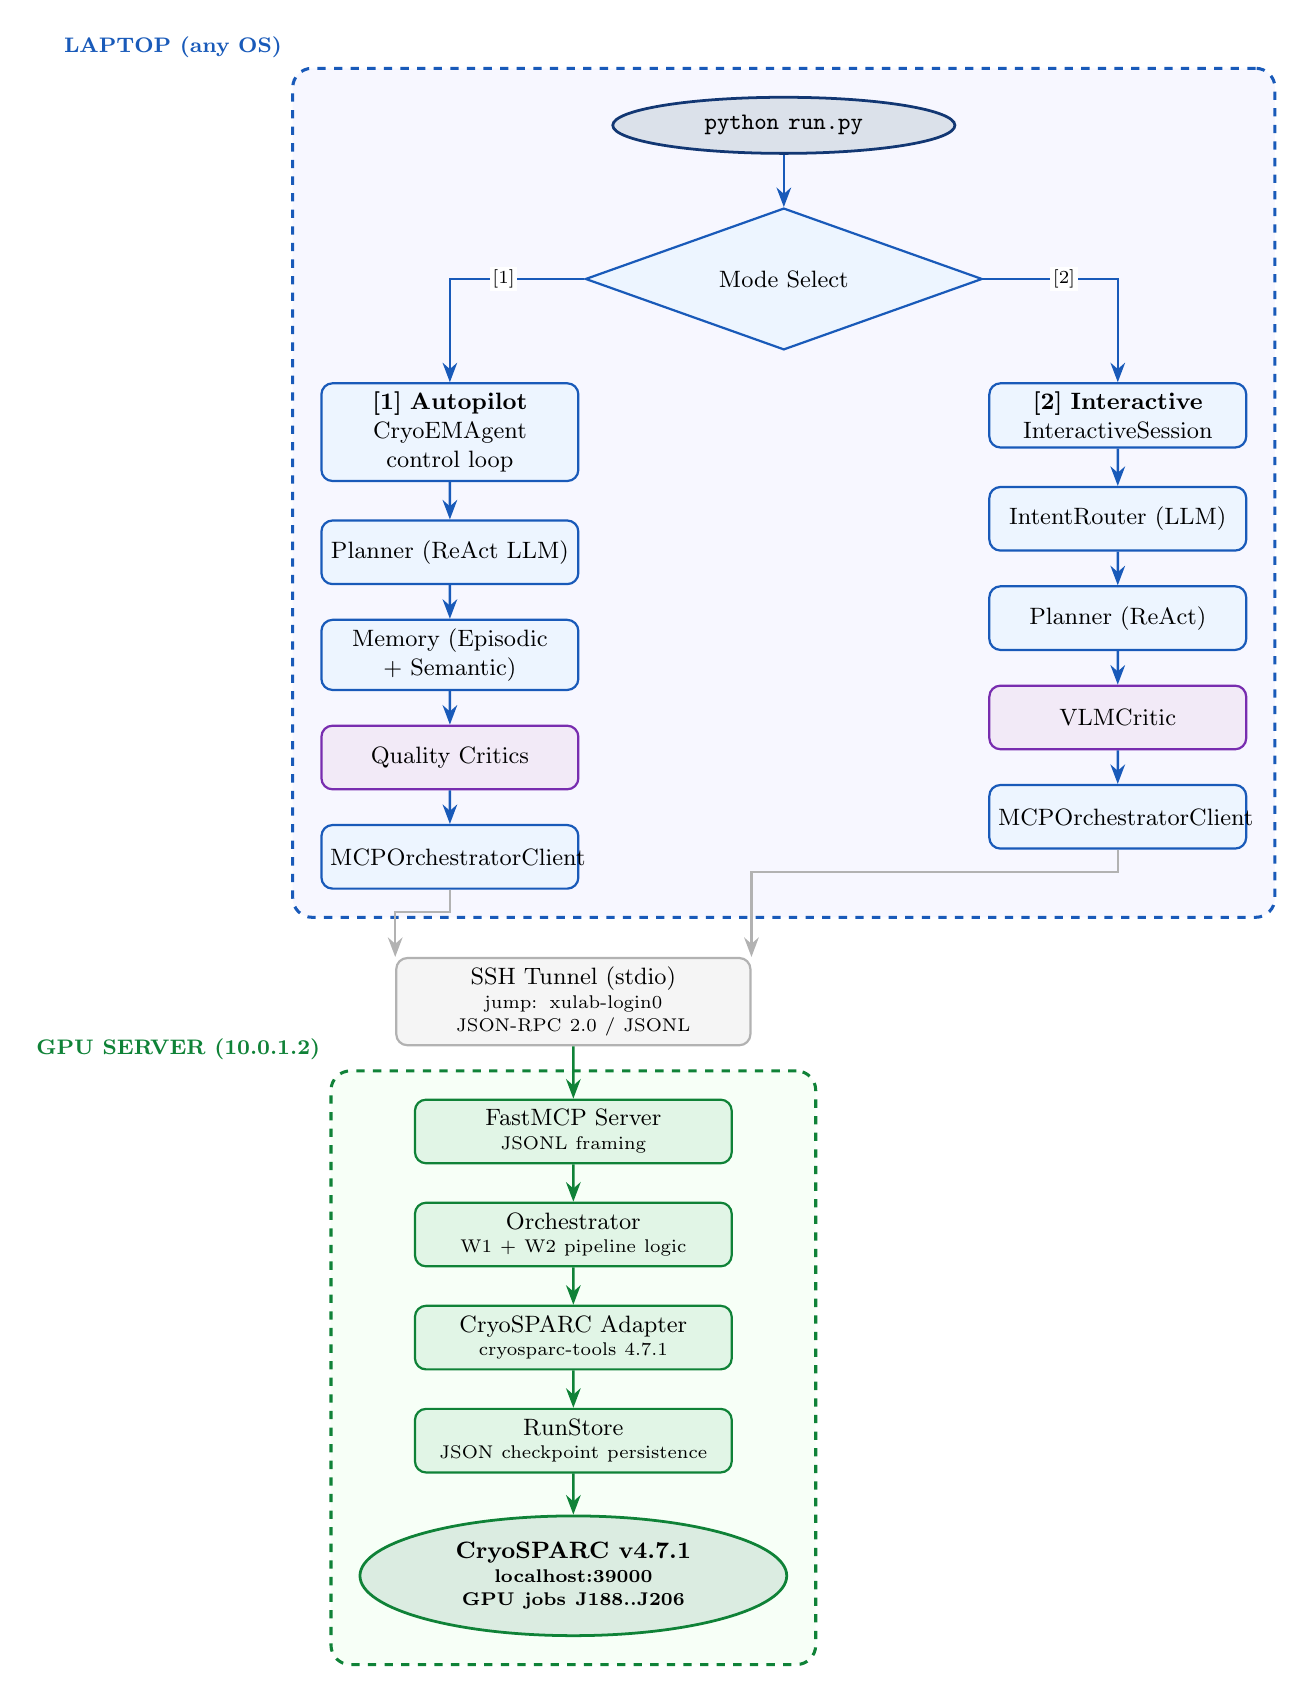
\begin{tikzpicture}[node distance=0.55cm and 1.8cm, scale=0.95,
                    transform shape]

  %% ── Laptop column ──────────────────────────────────────────────────────
  \node[termnode=titlebg, text width=3.0cm] (run)
    {\texttt{python run.py}};

  \node[decision=3.8cm, below=0.7cm of run] (modesel)
    {Mode Select};

  % Autopilot branch
  \node[block=3.2cm, below left=0.9cm and 1.4cm of modesel] (apilot)
    {\textbf{[1] Autopilot}\\CryoEMAgent\\control loop};
  \node[block=3.2cm, below=0.5cm of apilot] (ap_planner)
    {Planner (ReAct LLM)};
  \node[block=3.2cm, below=0.45cm of ap_planner] (ap_mem)
    {Memory (Episodic + Semantic)};
  \node[vlmblock=3.2cm, below=0.45cm of ap_mem] (ap_vlm)
    {Quality Critics};
  \node[block=3.2cm, below=0.45cm of ap_vlm] (ap_mcp)
    {MCPOrchestratorClient};

  % Interactive branch
  \node[block=3.2cm, below right=0.9cm and 1.4cm of modesel] (inter)
    {\textbf{[2] Interactive}\\InteractiveSession};
  \node[block=3.2cm, below=0.5cm of inter] (in_router)
    {IntentRouter (LLM)};
  \node[block=3.2cm, below=0.45cm of in_router] (in_planner)
    {Planner (ReAct)};
  \node[vlmblock=3.2cm, below=0.45cm of in_planner] (in_vlm)
    {VLMCritic};
  \node[block=3.2cm, below=0.45cm of in_vlm] (in_mcp)
    {MCPOrchestratorClient};

  %% ── Background boxes for laptop ───────────────────────────────────────
  \begin{pgfonlayer}{background}
    \node[bbox=agentblue, fill=blue!3,
          fit=(run)(modesel)(apilot)(ap_planner)(ap_mem)(ap_vlm)(ap_mcp)
              (inter)(in_router)(in_planner)(in_vlm)(in_mcp),
          label={[font=\footnotesize\bfseries\color{agentblue}]
                 north west:LAPTOP (any OS)}] {};
  \end{pgfonlayer}

  %% ── SSH tunnel ─────────────────────────────────────────────────────────
  \node[block=4.5cm, below=0.9cm of ap_mcp, xshift=1.65cm,
        draw=gray!60, fill=gray!8] (ssh)
    {SSH Tunnel (stdio)\\[-2pt]
     {\scriptsize jump: xulab-login0}\\[-2pt]
     {\scriptsize JSON-RPC 2.0 / JSONL}};

  %% ── GPU server column ──────────────────────────────────────────────────
  \node[srvblock=4.0cm, below=0.7cm of ssh] (fastmcp)
    {FastMCP Server\\[-2pt]{\scriptsize JSONL framing}};
  \node[srvblock=4.0cm, below=0.5cm of fastmcp] (orch)
    {Orchestrator\\[-2pt]{\scriptsize W1 + W2 pipeline logic}};
  \node[srvblock=4.0cm, below=0.5cm of orch] (csadapter)
    {CryoSPARC Adapter\\[-2pt]{\scriptsize cryosparc-tools 4.7.1}};
  \node[srvblock=4.0cm, below=0.5cm of csadapter] (runstore)
    {RunStore\\[-2pt]{\scriptsize JSON checkpoint persistence}};
  \node[termnode=servergreen, below=0.55cm of runstore, text width=3.8cm]
    (cryosparc)
    {CryoSPARC v4.7.1\\[-2pt]{\scriptsize localhost:39000}\\[-2pt]
     {\scriptsize GPU jobs J188..J206}};

  \begin{pgfonlayer}{background}
    \node[bbox=servergreen, fill=green!3,
          fit=(fastmcp)(orch)(csadapter)(runstore)(cryosparc),
          label={[font=\footnotesize\bfseries\color{servergreen}]
                 north west:GPU SERVER (10.0.1.2)}] {};
  \end{pgfonlayer}

  %% ── Arrows ─────────────────────────────────────────────────────────────
  \draw[arrblu] (run) -- (modesel);
  \draw[arrblu] (modesel) -| node[lbl, pos=0.3]{[1]} (apilot);
  \draw[arrblu] (modesel) -| node[lbl, pos=0.3]{[2]} (inter);
  \draw[arrblu] (apilot)--(ap_planner);
  \draw[arrblu] (ap_planner)--(ap_mem);
  \draw[arrblu] (ap_mem)--(ap_vlm);
  \draw[arrblu] (ap_vlm)--(ap_mcp);
  \draw[arrblu] (inter)--(in_router);
  \draw[arrblu] (in_router)--(in_planner);
  \draw[arrblu] (in_planner)--(in_vlm);
  \draw[arrblu] (in_vlm)--(in_mcp);
  \draw[arr]    (ap_mcp.south) -- ++(0,-0.3) -| (ssh.north west);
  \draw[arr]    (in_mcp.south) -- ++(0,-0.3) -| (ssh.north east);
  \draw[arrgrn] (ssh)--(fastmcp);
  \draw[arrgrn] (fastmcp)--(orch);
  \draw[arrgrn] (orch)--(csadapter);
  \draw[arrgrn] (csadapter)--(runstore);
  \draw[arrgrn] (runstore)--(cryosparc);

\end{tikzpicture}
\caption{Full system architecture. The laptop houses the AI agent brain; the
GPU server runs the FastMCP server and CryoSPARC. Communication uses SSH stdio
with JSON-RPC 2.0 (JSONL framing) --- the same protocol as Cursor and Claude
Desktop MCP integrations.}
\label{fig:architecture}
\end{figure}

% ════════════════════════════════════════════════════════════════════════════
\section{Two Operating Modes}
\label{sec:modes}
% ════════════════════════════════════════════════════════════════════════════

CryoEMAgent presents a mode selector at launch and provides two distinct
interfaces over the \emph{same} MCP engine:

\begin{table}[H]
\centering
\caption{Feature comparison: Autopilot vs.\ Interactive mode}
\label{tab:modes}
\renewcommand{\arraystretch}{1.3}
\begin{tabularx}{\textwidth}{l X X}
\toprule
\textbf{Feature} & \textbf{Autopilot} & \textbf{Interactive} \\
\midrule
GPU steps         & Fully autonomous & Fully autonomous \\
Checkpoints       & Print instructions, wait ENTER
                  & VLM assessment + optional human review \\
LLM reasoning     & Written to JSON log file
                  & Shown live as Rich TUI panels \\
User input        & Press ENTER to resume
                  & Natural language conversation \\
Progress display  & Basic step counter
                  & Progress bar + live pipeline table \\
Step narration    & Silent
                  & LLM explains each completed step \\
Intent routing    & Direct command parsing
                  & LLM intent classification (11 intents) \\
Best for          & Overnight production runs
                  & Demo, research, learning, fine control \\
\bottomrule
\end{tabularx}
\end{table}

\begin{figure}[H]
\centering
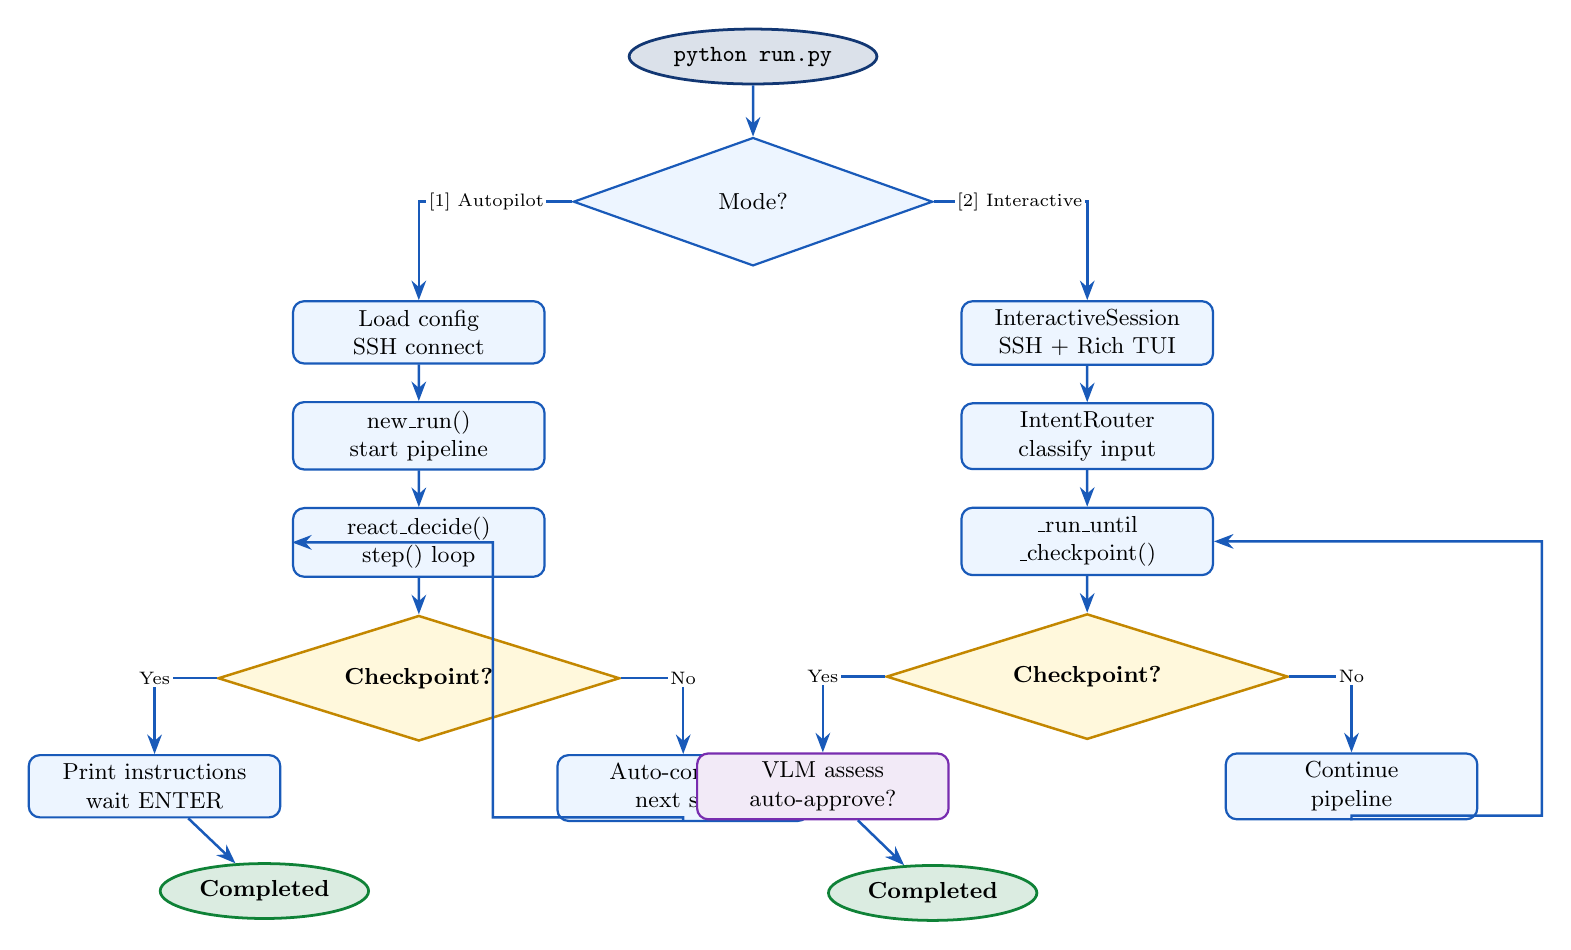
\begin{tikzpicture}[node distance=0.6cm and 1.6cm, scale=0.93,
                    transform shape]

  \node[termnode=titlebg] (entry) {\texttt{python run.py}};
  \node[decision=3.4cm, below=0.7cm of entry] (mq) {Mode?};

  %% Autopilot
  \node[block=3.2cm, below left=0.9cm and 1.6cm of mq] (a1)
    {Load config\\SSH connect};
  \node[block=3.2cm, below=0.5cm of a1] (a2)
    {new\_run()\\start pipeline};
  \node[block=3.2cm, below=0.5cm of a2] (a3)
    {react\_decide()\\step() loop};
  \node[cpblock=3.6cm, below=0.5cm of a3] (a4) {Checkpoint?};
  \node[block=3.2cm, below left=0.6cm and 0.5cm of a4] (a5)
    {Print instructions\\wait ENTER};
  \node[block=3.2cm, below right=0.6cm and 0.5cm of a4] (a6)
    {Auto-continue\\next step};
  \node[termnode=servergreen, below=0.6cm of a5, xshift=1.5cm] (adone)
    {Completed};

  %% Interactive
  \node[block=3.2cm, below right=0.9cm and 1.6cm of mq] (i1)
    {InteractiveSession\\SSH + Rich TUI};
  \node[block=3.2cm, below=0.5cm of i1] (i2)
    {IntentRouter\\classify input};
  \node[block=3.2cm, below=0.5cm of i2] (i3)
    {\_run\_until\\\_checkpoint()};
  \node[cpblock=3.6cm, below=0.5cm of i3] (i4) {Checkpoint?};
  \node[vlmblock=3.2cm, below left=0.6cm and 0.5cm of i4] (i5)
    {VLM assess\\auto-approve?};
  \node[block=3.2cm, below right=0.6cm and 0.5cm of i4] (i6)
    {Continue\\pipeline};
  \node[termnode=servergreen, below=0.6cm of i5, xshift=1.5cm] (idone)
    {Completed};

  \draw[arrblu] (entry)--(mq);
  \draw[arrblu] (mq) -| node[lbl, pos=0.28]{[1] Autopilot} (a1);
  \draw[arrblu] (mq) -| node[lbl, pos=0.28]{[2] Interactive} (i1);

  \draw[arrblu] (a1)--(a2);
  \draw[arrblu] (a2)--(a3);
  \draw[arrblu] (a3)--(a4);
  \draw[arrblu] (a4) -| node[lbl]{Yes} (a5);
  \draw[arrblu] (a4) -| node[lbl]{No} (a6);
  \draw[arrblu] (a5) -- (adone);
  \draw[arrblu] (a6) -- ++(0,-0.4) -- ++(-2.6,0) |- (a3.west);

  \draw[arrblu] (i1)--(i2);
  \draw[arrblu] (i2)--(i3);
  \draw[arrblu] (i3)--(i4);
  \draw[arrblu] (i4) -| node[lbl]{Yes} (i5);
  \draw[arrblu] (i4) -| node[lbl]{No} (i6);
  \draw[arrblu] (i5) -- (idone);
  \draw[arrblu] (i6) -- ++(0,-0.4) -- ++(2.6,0) |- (i3.east);

\end{tikzpicture}
\caption{Control flow for Autopilot and Interactive modes. Both share the same
MCP engine; the branching determines UI behaviour and checkpoint handling only.}
\label{fig:modes}
\end{figure}

% ════════════════════════════════════════════════════════════════════════════
\section{Agentic Framework: Planning \texorpdfstring{$\cdot$}{.} Memory \texorpdfstring{$\cdot$}{.} Action}
\label{sec:agent}
% ════════════════════════════════════════════════════════════════════════════

The agent implements a formal \textbf{Planning $\to$ Memory $\to$ Action}
loop at every pipeline step, grounded in the ReAct
framework~\cite{yao2023react}.

\subsection{Planning: ReAct Pattern}

At each step the LLM reasons through a four-field structured chain before
calling any tool:

\begin{tcolorbox}[
  colback=codebg, colframe=agentblue, arc=4pt, boxrule=0.8pt,
  title={\small\bfseries ReAct Reasoning Chain --- live example (step: patch\_ctf)}
]
\begin{lstlisting}[numbers=none, frame=none, backgroundcolor=\color{codebg}]
Observation:  patch_motion completed. 20 micrographs produced.
              Step executed without errors.

Thought:      Motion correction successful on all 20 micrographs.
              CTF estimation measures defocus and astigmatism per
              micrograph and is mandatory before particle picking.

Tool:         run_patch_ctf_estimation

Decision:     CONTINUE

Reasoning:    CTF estimation is the standard next step after motion
              correction. No quality flags raised. Proceeding.

Recommendation: Proceed to CTF estimation immediately.
\end{lstlisting}
\end{tcolorbox}

\subsubsection{Formal tool definitions}

The LLM system prompt contains \textbf{15 formally defined CryoSPARC tools},
each with \textit{name}, \textit{description}, \textit{when\_to\_use},
and \textit{outputs} fields:

\begin{table}[H]
\centering
\caption{CryoSPARC tool definitions injected into the LLM system prompt}
\label{tab:tools}
\small
\renewcommand{\arraystretch}{1.25}
\begin{tabular}{cl p{8.2cm}}
\toprule
\textbf{\#} & \textbf{Tool name} & \textbf{Description and trigger} \\
\midrule
1  & \texttt{run\_import\_movies}
   & Import raw .tif/.mrc movies into the CryoSPARC workspace \\
2  & \texttt{run\_patch\_motion\_correction}
   & Patch-based frame alignment; removes beam-induced motion blur \\
3  & \texttt{run\_patch\_ctf\_estimation}
   & Estimate CTF parameters (defocus, astigmatism) per micrograph \\
4  & \texttt{curate\_exposures}
   & \textbf{[CP]} Expert review: remove low-quality micrographs \\
5  & \texttt{run\_blob\_picker}
   & Laplacian-of-Gaussian particle detection \\
6  & \texttt{inspect\_blob\_picks}
   & \textbf{[CP]} Filter picks by NCC score; remove false positives \\
7  & \texttt{extract\_particles}
   & Extract particle stacks (256\,px box for GPCR) \\
8  & \texttt{run\_2d\_classification}
   & 50-class 2D averaging for visual quality assessment \\
9  & \texttt{select\_2d\_classes}
   & \textbf{[CP]} Keep protein classes; discard junk/noise \\
10 & \texttt{run\_abinit\_reconstruction}
   & Ab-initio 3D model generation (no reference required) \\
11 & \texttt{run\_homogeneous\_refinement}
   & Single-conformation 3D refinement \\
12 & \texttt{run\_template\_picker}
   & Template-based picking using W1 2D class averages \\
13 & \texttt{inspect\_template\_picks}
   & \textbf{[CP]} Filter template picks; verify specificity gain \\
14 & \texttt{select\_2d\_template\_classes}
   & \textbf{[CP]} Final stringent 2D class selection \\
15 & \texttt{run\_nonuniform\_refinement}
   & High-resolution refinement targeting $\leq$3.5\,\AA \\
+  & \texttt{assess\_quality}
   & Evaluate current-step metrics against domain thresholds \\
+  & \texttt{escalate\_to\_human}
   & Halt pipeline; raise alert for critical quality failure \\
\bottomrule
\multicolumn{3}{l}{\small\textit{\textbf{[CP]} = human checkpoint step}}
\end{tabular}
\end{table}

\subsubsection{Decision framework}

\begin{table}[H]
\centering
\caption{LLM decision outcomes and trigger conditions}
\label{tab:decisions}
\renewcommand{\arraystretch}{1.3}
\begin{tabular}{l p{5.0cm} p{6.2cm}}
\toprule
\textbf{Decision} & \textbf{Meaning} & \textbf{Trigger condition} \\
\midrule
\texttt{CONTINUE}
  & Proceed with next tool
  & Default --- all quality metrics within acceptable threshold \\
\texttt{ADJUST}
  & Proceed but flag marginal quality in memory
  & Metrics borderline but not critical; recommend parameter review \\
\texttt{ESCALATE}
  & Stop pipeline; alert human
  & Resolution $>8$\,\AA{} + particles $<1000$; OR 3+ consecutive
    step failures \\
\bottomrule
\end{tabular}
\end{table}

\subsection{Memory}

Two memory systems run in parallel throughout the pipeline.

\begin{figure}[H]
\centering
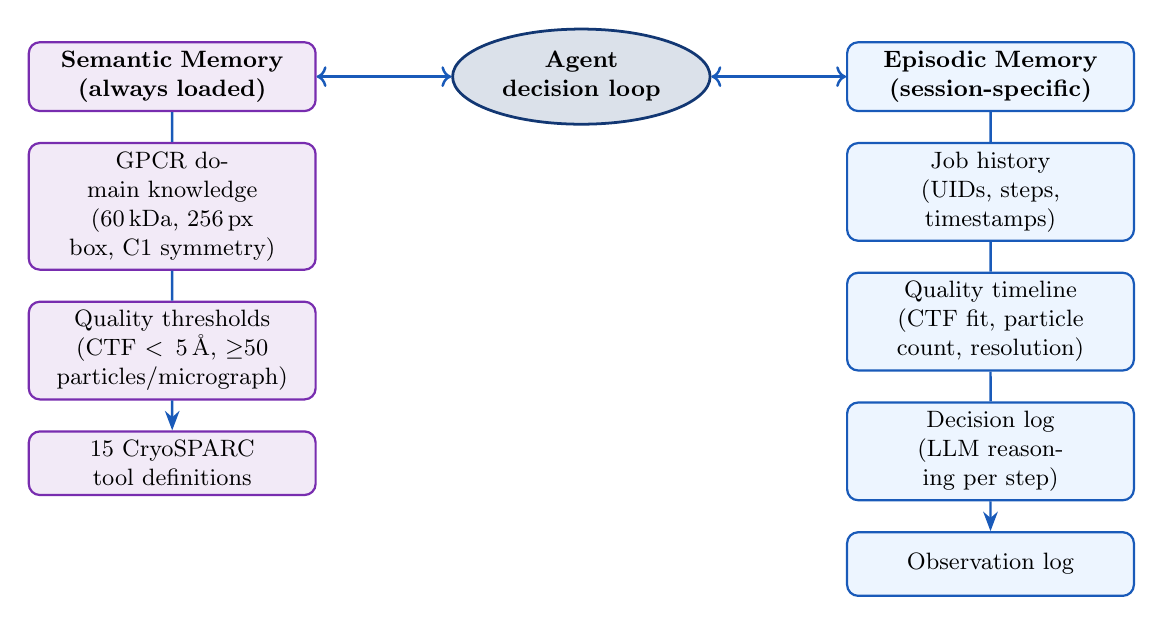
\begin{tikzpicture}[node distance=0.5cm and 1.5cm, scale=0.95,
                    transform shape]

  \node[termnode=titlebg, text width=2.2cm] (agent)
    {Agent\\decision loop};

  % Episodic memory (right)
  \node[block=3.6cm, right=1.8cm of agent] (ep_hdr)
    {\bfseries Episodic Memory\\(session-specific)};
  \node[block=3.6cm, below=0.4cm of ep_hdr] (ep1)
    {Job history\\(UIDs, steps, timestamps)};
  \node[block=3.6cm, below=0.4cm of ep1] (ep2)
    {Quality timeline\\(CTF fit, particle count, resolution)};
  \node[block=3.6cm, below=0.4cm of ep2] (ep3)
    {Decision log\\(LLM reasoning per step)};
  \node[block=3.6cm, below=0.4cm of ep3] (ep4)
    {Observation log};

  % Semantic memory (left)
  \node[vlmblock=3.6cm, left=1.8cm of agent] (sem_hdr)
    {\bfseries Semantic Memory\\(always loaded)};
  \node[vlmblock=3.6cm, below=0.4cm of sem_hdr] (sem1)
    {GPCR domain knowledge\\(60\,kDa, 256\,px box, C1 symmetry)};
  \node[vlmblock=3.6cm, below=0.4cm of sem1] (sem2)
    {Quality thresholds\\(CTF $<5$\,\AA, $\geq$50 particles/micrograph)};
  \node[vlmblock=3.6cm, below=0.4cm of sem2] (sem3)
    {15 CryoSPARC tool definitions};

  % Arrows
  \draw[arrblu, <->] (agent) -- (ep_hdr);
  \draw[arrblu, <->] (agent) -- (sem_hdr);
  \draw[arrblu] (ep_hdr)--(ep1)--(ep2)--(ep3)--(ep4);
  \draw[arrblu] (sem_hdr)--(sem1)--(sem2)--(sem3);

\end{tikzpicture}
\caption{Two-tier memory system. Episodic memory accumulates within a session;
semantic memory contains static GPCR domain knowledge loaded at startup.}
\label{fig:memory}
\end{figure}

\subsection{Action: MCP Tool Calls}

All pipeline actions are transmitted as \textbf{MCP tool calls} over SSH stdio:

\begin{table}[H]
\centering
\caption{Agent methods and their MCP tool mappings}
\label{tab:actions}
\renewcommand{\arraystretch}{1.3}
\begin{tabular}{l l p{6.2cm}}
\toprule
\textbf{Agent method} & \textbf{MCP tool} & \textbf{Effect on GPU server} \\
\midrule
\texttt{new\_run()}           & \texttt{cs\_start\_pipeline}
  & Initialise pipeline; launch first CryoSPARC job \\
\texttt{step()}               & \texttt{cs\_continue\_pipeline}
  & Advance one step; wait for GPU job completion \\
\texttt{resume\_checkpoint()} & \texttt{cs\_resume\_pipeline}
  & Resume pipeline after human has finished checkpoint \\
\texttt{load\_state()}        & \texttt{cs\_pipeline\_status}
  & Poll current job state and metrics \\
\texttt{write\_report()}      & \texttt{cs\_pipeline\_report}
  & Generate markdown + JSON run report \\
\texttt{list\_runs()}         & \texttt{cs\_list\_runs}
  & List all persisted runs in RunStore \\
\texttt{validate\_inputs()}   & \texttt{cs\_validate\_data\_source}
  & Pre-flight validation of data paths and config \\
\bottomrule
\end{tabular}
\end{table}

% ════════════════════════════════════════════════════════════════════════════
\section{VLM Critic: Intelligent Checkpoint Evaluation}
\label{sec:vlm}
% ════════════════════════════════════════════════════════════════════════════

\subsection{Design and Two-Tier Architecture}

The VLM critic (\texttt{cryoemagent/vlm\_critic.py}) replaces or assists
human judgment at the 5 checkpoint steps.

\begin{table}[H]
\centering
\caption{VLM critic evaluation tiers}
\label{tab:vlm-tiers}
\renewcommand{\arraystretch}{1.3}
\begin{tabular}{l l l p{5.8cm}}
\toprule
\textbf{Tier} & \textbf{Works in} & \textbf{Input} & \textbf{Method} \\
\midrule
Tier 1 --- Metrics
  & Always (incl.\ remote SSH)
  & CryoSPARC job metrics: CTF fit, particle counts, acceptance rates
  & LLM reasons from numbers; no image required \\
\addlinespace
Tier 2 --- Vision
  & Local mode only
  & Actual micrograph / CTF plot / 2D class images
  & GPT-4V or Claude Vision API inspects images \\
\bottomrule
\end{tabular}
\end{table}

\subsection{Auto-Approval Flow}

\begin{figure}[H]
\centering
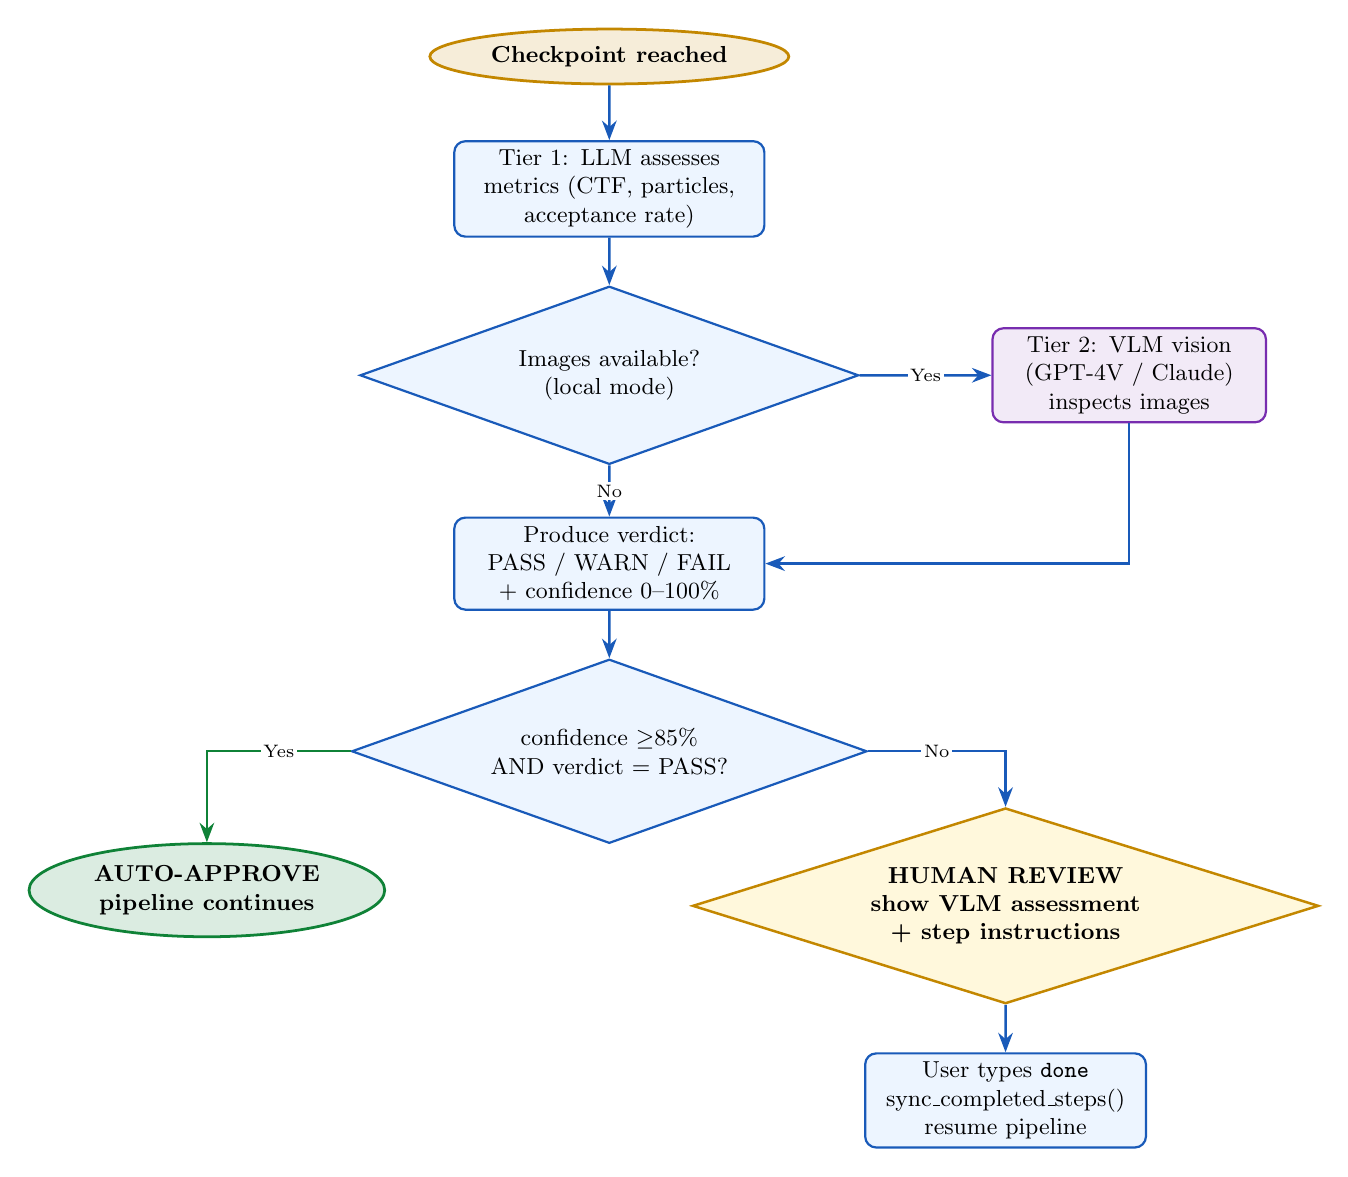
\begin{tikzpicture}[node distance=0.65cm and 1.8cm, scale=0.93,
                    transform shape]

  \node[termnode=checkpointyellow] (cp) {Checkpoint reached};

  \node[block=4.0cm, below=0.75cm of cp] (t1)
    {Tier 1: LLM assesses\\metrics (CTF, particles,\\acceptance rate)};

  \node[decision=4.0cm, below=0.65cm of t1] (imgq)
    {Images available?\\(local mode)};

  \node[vlmblock=3.5cm, right=1.8cm of imgq] (t2)
    {Tier 2: VLM vision\\(GPT-4V / Claude)\\inspects images};

  \node[block=4.0cm, below=0.7cm of imgq] (assess)
    {Produce verdict:\\PASS / WARN / FAIL\\+ confidence 0--100\%};

  \node[decision=4.4cm, below=0.65cm of assess] (autoq)
    {confidence $\geq$85\%\\AND verdict = PASS?};

  \node[termnode=servergreen, below left=0.8cm and 2.0cm of autoq,
        text width=3.2cm] (autoappr)
    {\textbf{AUTO-APPROVE}\\pipeline continues};

  \node[cpblock=4.2cm, below right=0.8cm and 1.5cm of autoq] (humanreview)
    {HUMAN REVIEW\\show VLM assessment\\+ step instructions};

  \node[block=3.6cm, below=0.65cm of humanreview] (userdone)
    {User types \texttt{done}\\sync\_completed\_steps()\\resume pipeline};

  % Arrows
  \draw[arrblu] (cp)--(t1);
  \draw[arrblu] (t1)--(imgq);
  \draw[arrblu] (imgq) -- node[lbl]{No} (assess);
  \draw[arrblu] (imgq) -- node[lbl]{Yes} (t2);
  \draw[arrblu] (t2) |- (assess);
  \draw[arrblu] (assess)--(autoq);
  \draw[arrgrn] (autoq) -| node[lbl, pos=0.25]{Yes} (autoappr);
  \draw[arrblu] (autoq) -| node[lbl, pos=0.25]{No}  (humanreview);
  \draw[arrblu] (humanreview)--(userdone);

\end{tikzpicture}
\caption{VLM checkpoint evaluation flow. Tier 1 always runs (metrics
reasoning); Tier 2 activates when images are locally available.
Auto-approval at $\geq$85\% confidence eliminates the human bottleneck for
high-quality data.}
\label{fig:vlm}
\end{figure}

\subsection{VLM Output Structure}

\begin{lstlisting}[language=Python,
  caption={VLMAssessment dataclass (cryoemagent/vlm\_critic.py)},
  label=lst:vlm-assessment]
@dataclass
class VLMAssessment:
    step:               str       # e.g. "curate"
    verdict:            str       # "PASS" | "WARN" | "FAIL"
    decision:           str       # "approve" | "approve_with_adjustments"
                                  #           | "escalate_to_human"
    confidence:         float     # 0.0 -- 1.0
    auto_approved:      bool      # True if confidence >= 0.85 and PASS
    observations:       List[str]
    reasoning:          str
    recommended_actions: List[str]
    suggested_params:   Dict[str, Any]
    used_images:        bool      # True = Tier 2 was used
\end{lstlisting}

\subsection{Checkpoint-Specific Evaluation Criteria}

\begin{table}[H]
\centering
\caption{GPCR-specific VLM evaluation criteria per checkpoint}
\label{tab:vlm-criteria}
\small
\renewcommand{\arraystretch}{1.35}
\begin{tabular}{l p{10.2cm}}
\toprule
\textbf{Checkpoint} & \textbf{VLM evaluates} \\
\midrule
\texttt{curate}
  & CTF fit: $<5$\,\AA\ (GOOD), $5$--$7$\,\AA\ (WARN), $>7$\,\AA\ (FAIL);
    ice thickness ratio; micrograph acceptance rate $\geq$70\%;
    defocus range $0.5$--$3.0$\,\textmu m underfocus \\
\addlinespace
\texttt{inspect\_blob}
  & Particles per micrograph: $\geq$50 (GOOD), 20--50 (WARN), $<$20 (FAIL);
    NCC score distribution (should be right-skewed);
    false-positive rate (carbon edges, ice crystals);
    pick density and particle centering \\
\addlinespace
\texttt{select2d\_blob}
  & Secondary structure visibility ($\alpha$-helices as lines in 2D classes);
    GPCR particle diameter 100--150\,\AA;
    orientation diversity (top, side, tilted views);
    absence of junk classes (ice rings, noise aggregates) \\
\addlinespace
\texttt{inspect\_template}
  & Template correlation score distribution (narrow, right-skewed);
    particles per micrograph $\geq$50;
    false positive rate vs.\ blob picking (should be lower) \\
\addlinespace
\texttt{select2d\_template}
  & Transmembrane (TM) helix density visible in selected classes;
    orientation diversity including tilted views;
    particle retention 40--60\%;
    total particle count $\geq$10\,000 for reliable ab-initio reconstruction \\
\bottomrule
\end{tabular}
\end{table}

% ════════════════════════════════════════════════════════════════════════════
\section{Pipeline: W1\,+\,W2 (19 Steps)}
\label{sec:pipeline}
% ════════════════════════════════════════════════════════════════════════════

\subsection{Design Rationale}

The full cryo-EM processing pipeline consists of two sequential sub-pipelines:

\begin{itemize}[leftmargin=1.6em, itemsep=3pt]
  \item \textbf{W1 --- Blob Pipeline} (steps 1--11): conventional
        Laplacian-of-Gaussian blob-based particle detection.
        Produces an initial reference-free ab-initio 3D model.
  \item \textbf{W2 --- Template Pipeline} (steps 12--19): higher-accuracy
        template-based picking using the 2D class averages from W1 as
        templates.  Produces the final high-resolution structure
        ($\leq$3.5\,\AA\ target).
\end{itemize}

\subsection{Complete Pipeline Table}

\begin{longtable}{
  >{\centering\arraybackslash}p{0.5cm}
  >{\centering\arraybackslash}p{0.7cm}
  p{4.2cm}
  p{3.4cm}
  >{\centering\arraybackslash}p{1.6cm}
  >{\centering\arraybackslash}p{1.5cm}
}
\caption{Full W1\,+\,W2 pipeline --- 19 steps with checkpoint markers}
\label{tab:pipeline}\\
\toprule
\textbf{\#} & \textbf{Wave} & \textbf{Step label}
  & \textbf{Key} & \textbf{Human CP} & \textbf{GPU job} \\
\midrule
\endfirsthead
\multicolumn{6}{l}{\small\itshape (continued from previous page)}\\
\toprule
\textbf{\#} & \textbf{Wave} & \textbf{Step label}
  & \textbf{Key} & \textbf{Human CP} & \textbf{GPU job} \\
\midrule
\endhead
\midrule
\multicolumn{6}{r}{\small\itshape (continued on next page)}\\
\endfoot
\bottomrule
\endlastfoot

% W1 rows
\rowcolor{w1color}
1  & W1 & Import Movies                & \texttt{import\_movies}    &            & J188 \\
\rowcolor{w1color}
2  & W1 & Patch Motion Correction      & \texttt{patch\_motion}     &            & J189 \\
\rowcolor{w1color}
3  & W1 & Patch CTF Estimation         & \texttt{patch\_ctf}        &            & J190 \\
\rowcolor{cpcolor}
4  & W1 & \textbf{Curate Exposures}    & \texttt{curate}
   & \textbf{Yes} & J191 \\
\rowcolor{w1color}
5  & W1 & Blob Picker                  & \texttt{blob\_pick}        &            & J192 \\
\rowcolor{cpcolor}
6  & W1 & \textbf{Inspect Blob Picks}  & \texttt{inspect\_blob}
   & \textbf{Yes} & J193 \\
\rowcolor{w1color}
7  & W1 & Extract Particles (Blob)     & \texttt{extract\_blob}     &            & J194 \\
\rowcolor{w1color}
8  & W1 & 2D Classification (Blob)     & \texttt{class2d\_blob}     &            & J195 \\
\rowcolor{cpcolor}
9  & W1 & \textbf{Select 2D Classes (Blob)} & \texttt{select2d\_blob}
   & \textbf{Yes} & J196 \\
\rowcolor{w1color}
10 & W1 & Ab-initio Reconstruction     & \texttt{abinit\_blob}      &            & J197 \\
\rowcolor{w1color}
11 & W1 & Homogeneous Refinement       & \texttt{homo\_blob}        &            & J198 \\
\midrule
\multicolumn{6}{c}{\cellcolor{gray!12}
  \textbf{W1 complete --- 2D class averages feed into W2 as templates}} \\
\midrule
\rowcolor{w2color}
12 & W2 & Template Picker              & \texttt{template\_pick}    &            & J199 \\
\rowcolor{cpcolor}
13 & W2 & \textbf{Inspect Template Picks} & \texttt{inspect\_template}
   & \textbf{Yes} & J200 \\
\rowcolor{w2color}
14 & W2 & Extract Particles (Template) & \texttt{extract\_template} &            & J201 \\
\rowcolor{w2color}
15 & W2 & 2D Classification (Template) & \texttt{class2d\_template} &            & J202 \\
\rowcolor{cpcolor}
16 & W2 & \textbf{Select 2D Classes (Template)} & \texttt{select2d\_template}
   & \textbf{Yes} & J203 \\
\rowcolor{w2color}
17 & W2 & Ab-initio (Template)         & \texttt{abinit\_template}  &            & J204 \\
\rowcolor{w2color}
18 & W2 & Homogeneous Refinement (W2)  & \texttt{homo\_template}    &            & J205 \\
\rowcolor{w2color}
19 & W2 & \textbf{Non-uniform Refinement} & \texttt{nonuniform\_template}
   &            & J206 \\
\end{longtable}

\medskip
\noindent
\colorbox{w1color}{\rule{0pt}{6pt}\hspace{4pt}} W1 Blob Pipeline\quad
\colorbox{w2color}{\rule{0pt}{6pt}\hspace{4pt}} W2 Template Pipeline\quad
\colorbox{cpcolor}{\rule{0pt}{6pt}\hspace{4pt}} Human Checkpoint (VLM evaluates first)

\subsection{Pipeline Flow Diagram}

\begin{figure}[H]
\centering
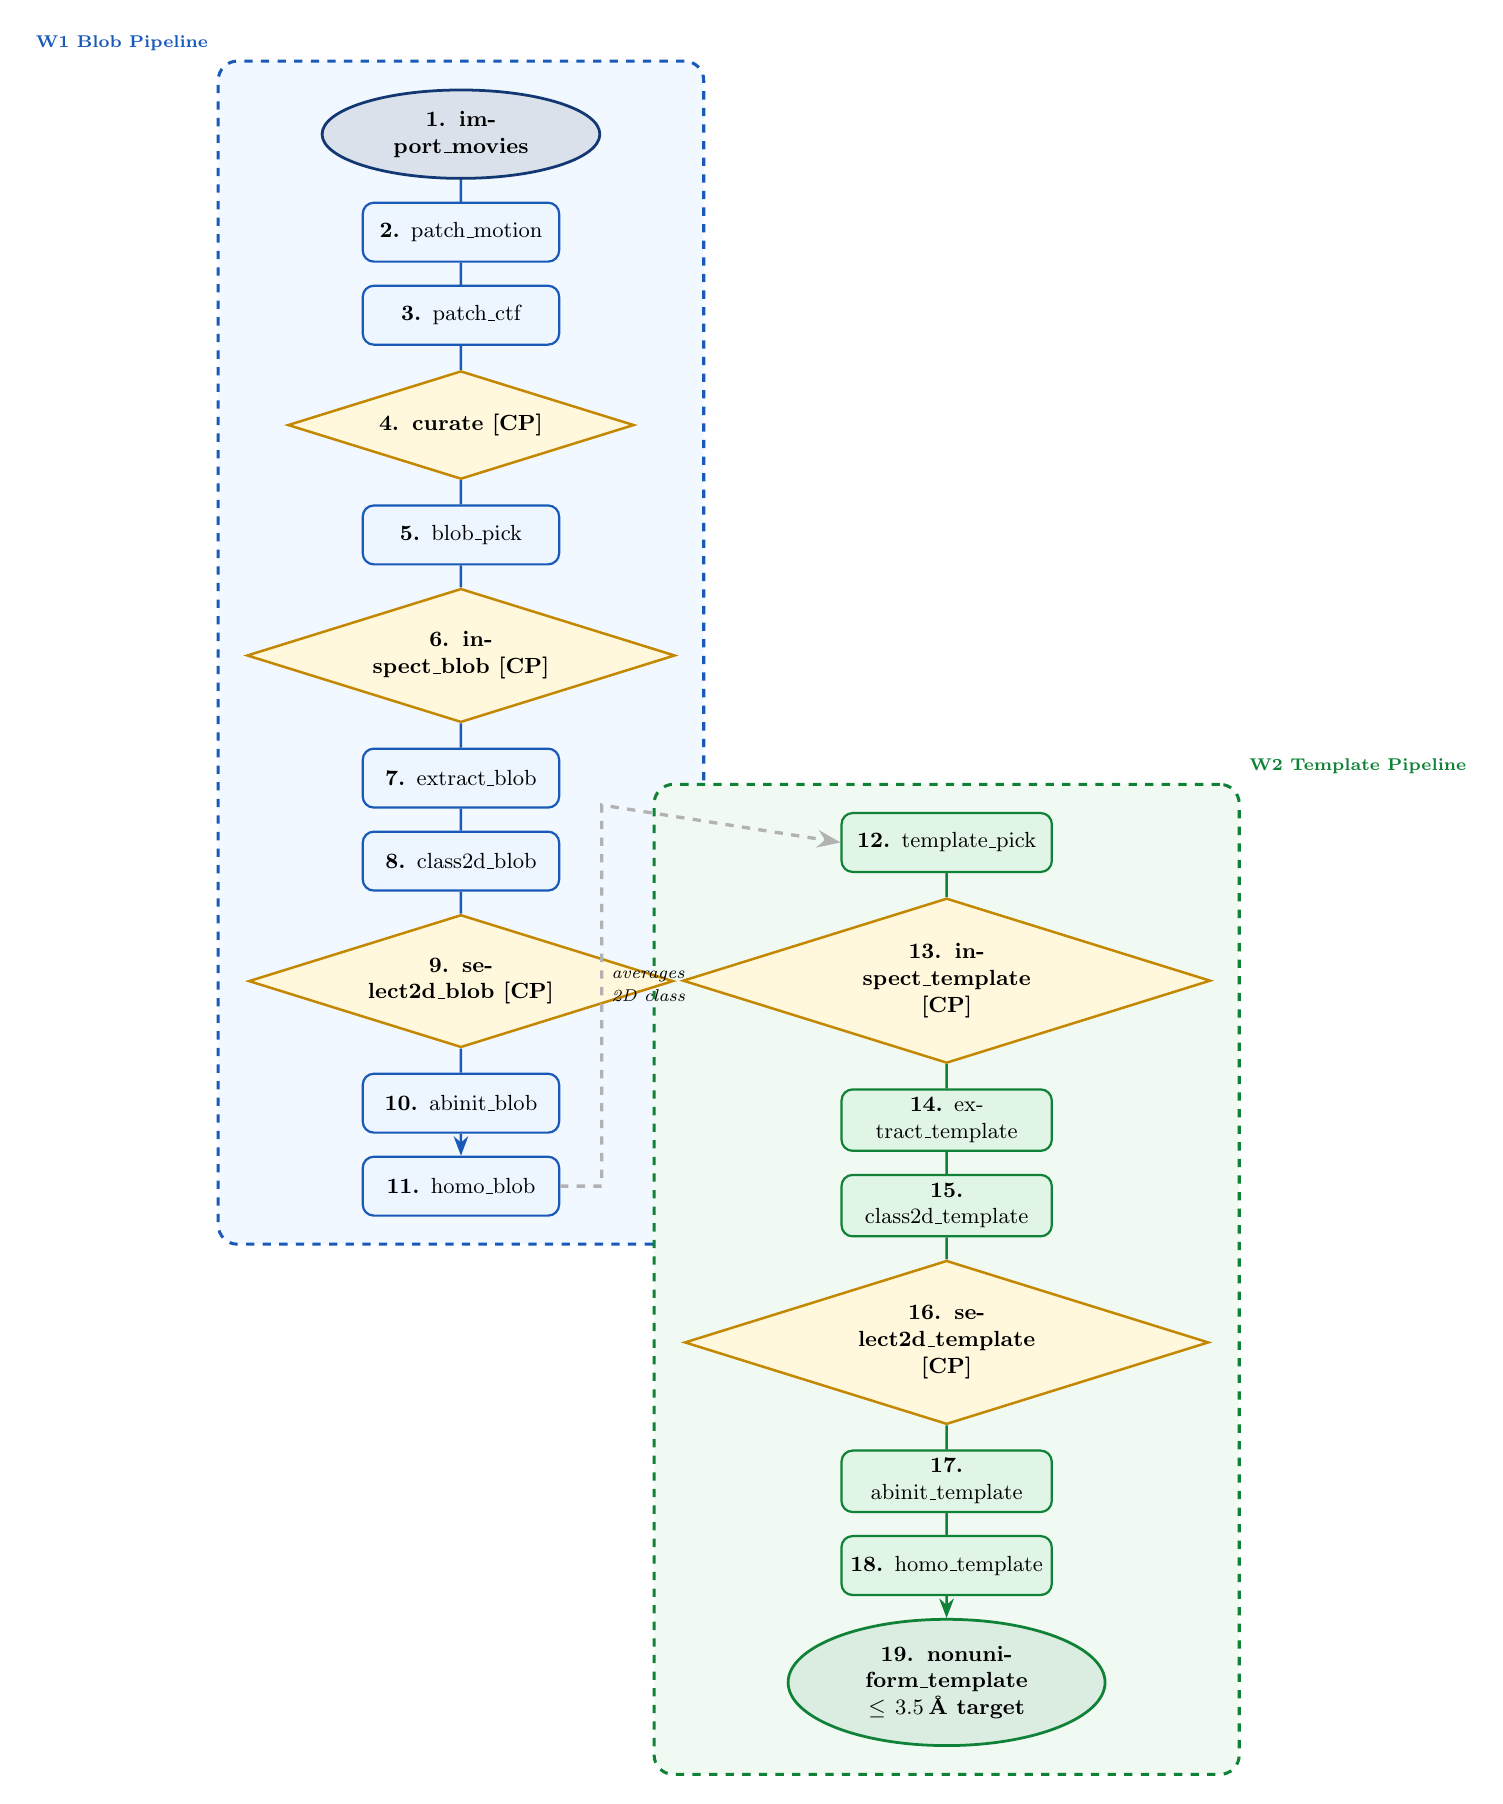
\begin{tikzpicture}[
  node distance = 0.38cm and 2.4cm,
  every node/.style = {font=\scriptsize},
  scale = 0.88, transform shape
]

  %% W1 column
  \node[termnode=titlebg, text width=2.6cm] (s1)  {\textbf{1.} import\_movies};
  \node[block=2.6cm, below=0.32cm of s1]    (s2)  {\textbf{2.} patch\_motion};
  \node[block=2.6cm, below=0.32cm of s2]    (s3)  {\textbf{3.} patch\_ctf};
  \node[cpblock=3.0cm, below=0.35cm of s3]  (s4)  {\textbf{4.} curate \textbf{[CP]}};
  \node[block=2.6cm, below=0.35cm of s4]    (s5)  {\textbf{5.} blob\_pick};
  \node[cpblock=3.0cm, below=0.32cm of s5]  (s6)  {\textbf{6.} inspect\_blob \textbf{[CP]}};
  \node[block=2.6cm, below=0.35cm of s6]    (s7)  {\textbf{7.} extract\_blob};
  \node[block=2.6cm, below=0.32cm of s7]    (s8)  {\textbf{8.} class2d\_blob};
  \node[cpblock=3.0cm, below=0.32cm of s8]  (s9)  {\textbf{9.} select2d\_blob \textbf{[CP]}};
  \node[block=2.6cm, below=0.35cm of s9]    (s10) {\textbf{10.} abinit\_blob};
  \node[block=2.6cm, below=0.32cm of s10]   (s11) {\textbf{11.} homo\_blob};

  %% W2 column
  \node[srvblock=2.8cm, right=2.4cm of s9, yshift=2.0cm] (s12)
    {\textbf{12.} template\_pick};
  \node[cpblock=3.2cm, below=0.35cm of s12] (s13)
    {\textbf{13.} inspect\_template \textbf{[CP]}};
  \node[srvblock=2.8cm, below=0.35cm of s13] (s14)
    {\textbf{14.} extract\_template};
  \node[srvblock=2.8cm, below=0.32cm of s14] (s15)
    {\textbf{15.} class2d\_template};
  \node[cpblock=3.2cm, below=0.32cm of s15]  (s16)
    {\textbf{16.} select2d\_template \textbf{[CP]}};
  \node[srvblock=2.8cm, below=0.35cm of s16] (s17)
    {\textbf{17.} abinit\_template};
  \node[srvblock=2.8cm, below=0.32cm of s17] (s18)
    {\textbf{18.} homo\_template};
  \node[termnode=servergreen, below=0.32cm of s18, text width=3.0cm] (s19)
    {\textbf{19.} nonuniform\_template\\$\leq3.5$\,\AA\ target};

  %% W1 arrows
  \draw[arrblu] (s1)--(s2)--(s3)--(s4)--(s5)--(s6)
                   --(s7)--(s8)--(s9)--(s10)--(s11);

  %% W2 arrows
  \draw[arrgrn] (s12)--(s13)--(s14)--(s15)--(s16)--(s17)--(s18)--(s19);

  %% W1 -> W2 bridge
  \draw[arr, dashed, very thick]
    (s11.east) -- ++(0.6,0)
    -- ++(0, 5.5)
    node[midway, right, font=\scriptsize\itshape]{2D class}
    node[pos=0.55, right, font=\scriptsize\itshape]{averages}
    -- (s12.west);

  %% Labels
  \begin{pgfonlayer}{background}
    \node[bbox=agentblue, fill=w1color!50,
          fit=(s1)(s2)(s3)(s4)(s5)(s6)(s7)(s8)(s9)(s10)(s11),
          label={[font=\scriptsize\bfseries\color{agentblue}]
                 north west:W1 Blob Pipeline}] {};
    \node[bbox=servergreen, fill=w2color!50,
          fit=(s12)(s13)(s14)(s15)(s16)(s17)(s18)(s19),
          label={[font=\scriptsize\bfseries\color{servergreen}]
                 north east:W2 Template Pipeline}] {};
  \end{pgfonlayer}

\end{tikzpicture}
\caption{W1\,+\,W2 pipeline flowchart. Yellow diamonds are the 5 human
checkpoints (\textbf{[CP]}) where the VLM critic evaluates quality.
W1 2D class averages are passed as templates to the W2 picker, enabling
higher-accuracy particle detection in the second wave.}
\label{fig:pipeline}
\end{figure}

\subsection{Quality Thresholds}

\begin{table}[H]
\centering
\caption{GPCR-specific quality thresholds used by VLM critic and LLM planner}
\label{tab:quality}
\renewcommand{\arraystretch}{1.3}
\begin{tabular}{l p{3.6cm} p{3.6cm} p{3.6cm}}
\toprule
\textbf{Metric}
  & \cellcolor{green!15}\textbf{GOOD}
  & \cellcolor{yellow!20}\textbf{WARN}
  & \cellcolor{red!12}\textbf{FAIL} \\
\midrule
CTF fit resolution
  & $<5$\,\AA
  & $5$--$7$\,\AA
  & $>7$\,\AA \\
Micrograph acceptance rate
  & $>70\%$
  & $50$--$70\%$
  & $<50\%$ \\
Particles per micrograph
  & $>50$
  & $20$--$50$
  & $<20$ \\
Final resolution
  & $\leq3.5$\,\AA
  & $3.5$--$5.0$\,\AA
  & $>5.0$\,\AA \\
\bottomrule
\end{tabular}
\end{table}

% ════════════════════════════════════════════════════════════════════════════
\section{MCP over SSH Architecture}
\label{sec:mcp}
% ════════════════════════════════════════════════════════════════════════════

\subsection{Protocol Design}

The agent communicates with the GPU server using \textbf{Model Context
Protocol (MCP)} --- the same JSON-RPC 2.0 protocol used by Cursor and
Claude Desktop.

\begin{figure}[H]
\centering
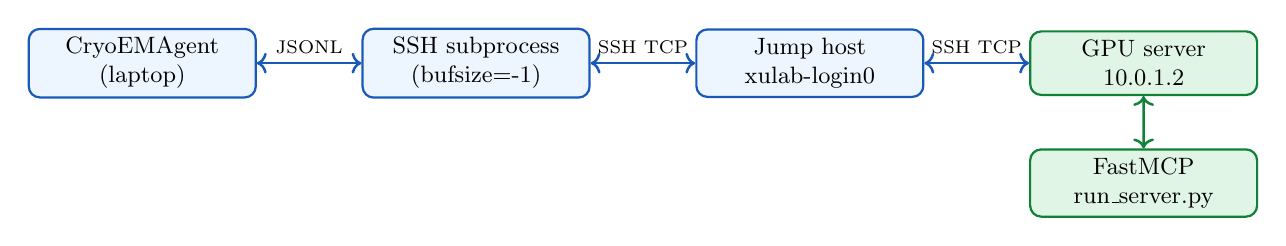
\begin{tikzpicture}[node distance=0.55cm and 1.4cm, scale=0.95,
                    transform shape]

  \node[block=2.8cm] (laptop)    {CryoEMAgent\\(laptop)};
  \node[block=2.8cm, right=1.4cm of laptop] (sshin) {SSH subprocess\\(bufsize=-1)};
  \node[block=2.8cm, right=1.4cm of sshin]  (jump)  {Jump host\\xulab-login0};
  \node[srvblock=2.8cm, right=1.4cm of jump] (gpu)   {GPU server\\10.0.1.2};
  \node[srvblock=2.8cm, below=0.7cm of gpu]  (fmcp)  {FastMCP\\run\_server.py};

  \draw[arrblu, <->] (laptop) -- node[above, font=\scriptsize]{JSONL} (sshin);
  \draw[arrblu, <->] (sshin)  -- node[above, font=\scriptsize]{SSH TCP} (jump);
  \draw[arrblu, <->] (jump)   -- node[above, font=\scriptsize]{SSH TCP} (gpu);
  \draw[arrgrn, <->] (gpu)    -- (fmcp);

\end{tikzpicture}
\caption{MCP-over-SSH communication chain. The laptop spawns an SSH
subprocess and writes JSON-RPC 2.0 messages to its stdin as
newline-delimited JSON (JSONL). Non-JSON lines (SSH banners) are silently
skipped.}
\label{fig:mcp}
\end{figure}

\subsection{JSONL Message Framing}

\begin{lstlisting}[caption={JSONL framing --- request and response},
  label=lst:jsonl]
# Request  (laptop -> GPU server, written to SSH stdin)
{"jsonrpc":"2.0","id":1,"method":"tools/call",
 "params":{"name":"cs_continue_pipeline",
           "arguments":{"run_id":"f57bbb1e-...","steps":1}}}

# Response  (GPU server -> laptop, read from SSH stdout)
{"jsonrpc":"2.0","id":1,
 "result":{"step":"patch_motion","status":"running",
           "checkpoint":false}}
\end{lstlisting}

\subsection{Windows Compatibility Fix}

\begin{tcolorbox}[
  colback=red!5, colframe=codered, arc=4pt, boxrule=0.8pt,
  title={\small\bfseries Bug fixed: OSError on Windows --- \texttt{bufsize=0}}
]
\small
\textbf{Root cause:}
\texttt{subprocess.Popen(bufsize=0)} (unbuffered) is incompatible with
Windows named-pipe handles and raises
\texttt{OSError: [Errno 22] Invalid argument} on \texttt{stdin.write()}.

\medskip
\textbf{Fix:}
Changed \texttt{bufsize=0} $\to$ \texttt{bufsize=-1} (default system
buffering) in \texttt{MCPStdioClient.\_\_init\_\_}.
Since \texttt{flush()} is called after every write, correctness is
unaffected.
\end{tcolorbox}

% ════════════════════════════════════════════════════════════════════════════
\section{Interactive Mode: Conversation Flow}
\label{sec:interactive}
% ════════════════════════════════════════════════════════════════════════════

\subsection{Intent Routing}

User messages are classified by an LLM-backed intent router before dispatch
to the appropriate handler:

\begin{table}[H]
\centering
\caption{Interactive mode intent classes and handlers}
\label{tab:intents}
\renewcommand{\arraystretch}{1.3}
\begin{tabular}{l p{5.4cm} l}
\toprule
\textbf{Intent} & \textbf{Trigger phrases} & \textbf{Handler method} \\
\midrule
\texttt{start}
  & ``start a run'', ``begin'', ``go''
  & \texttt{\_handle\_start} \\
\texttt{confirm\_checkpoint}
  & ``done'', ``finished'', ``ok'', ``complete''
  & \texttt{\_handle\_confirm\_checkpoint} \\
\texttt{continue}
  & ``continue'', ``proceed'', ``next''
  & \texttt{\_handle\_continue} \\
\texttt{status}
  & ``status'', ``progress'', ``where are we''
  & \texttt{\_handle\_status} \\
\texttt{quality}
  & ``quality'', ``how good'', ``metrics''
  & \texttt{\_handle\_quality} \\
\texttt{adjust\_param}
  & ``change'', ``adjust'', ``set parameter''
  & \texttt{\_handle\_adjust} \\
\texttt{report}
  & ``report'', ``save'', ``export''
  & \texttt{\_handle\_report} \\
\texttt{pause}
  & ``pause'', ``stop'', ``hold''
  & \texttt{\_handle\_pause} \\
\texttt{resume}
  & ``resume'', ``load run''
  & \texttt{\_handle\_resume} \\
\texttt{quit}
  & ``quit'', ``exit'', ``q''
  & \texttt{\_handle\_quit} \\
\texttt{chat}
  & anything else (e.g.\ ``what is CTF?'')
  & conversational LLM response \\
\bottomrule
\end{tabular}
\end{table}

\subsection{Interactive Session Flow Diagram}

\begin{figure}[H]
\centering
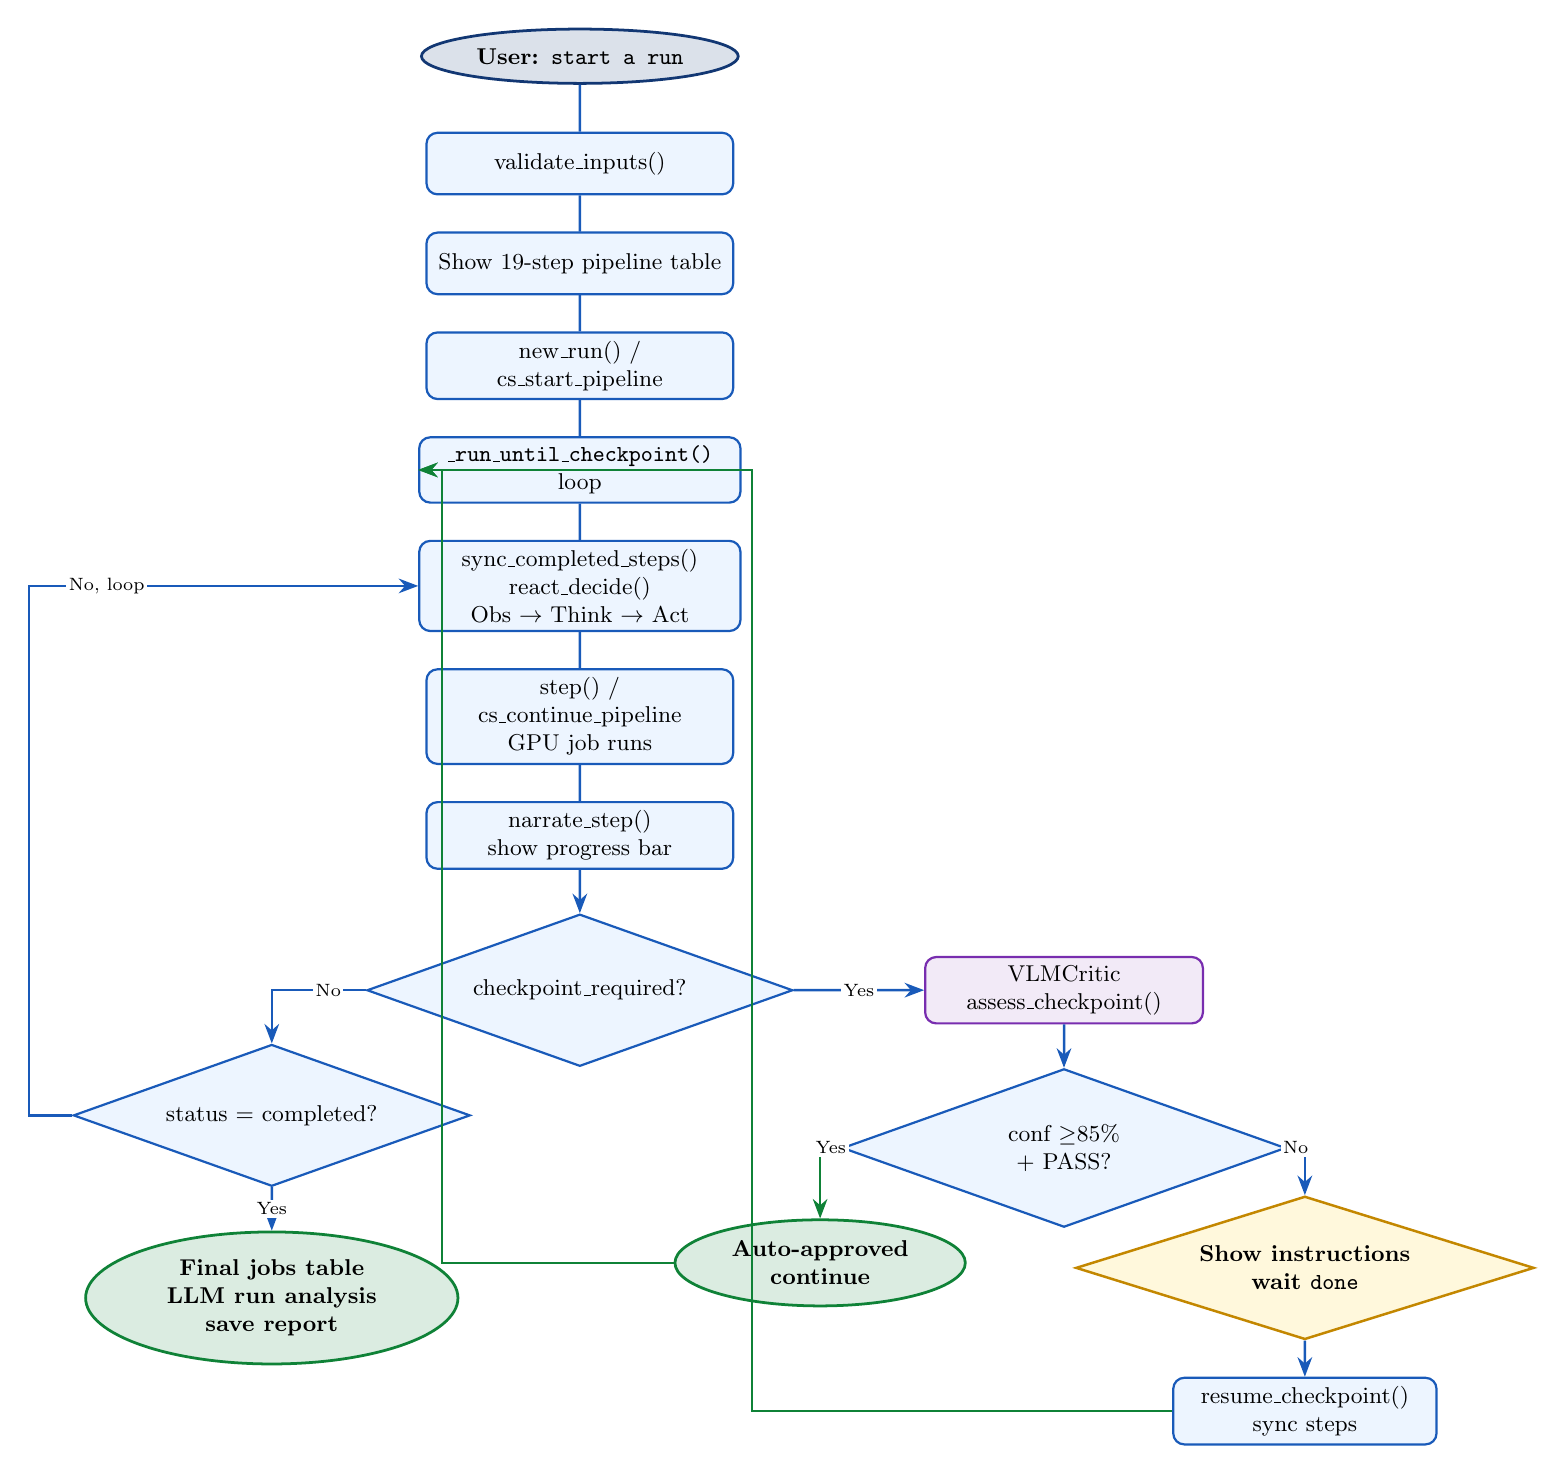
\begin{tikzpicture}[node distance=0.55cm and 1.8cm, scale=0.92,
                    transform shape]

  \node[termnode=titlebg] (u) {User: \texttt{start a run}};
  \node[block=4.0cm, below=0.65cm of u] (v)
    {validate\_inputs()};
  \node[block=4.0cm, below=0.5cm of v] (tbl)
    {Show 19-step pipeline table};
  \node[block=4.0cm, below=0.5cm of tbl] (nr)
    {new\_run() / cs\_start\_pipeline};
  \node[block=4.2cm, below=0.5cm of nr] (loop)
    {\texttt{\_run\_until\_checkpoint()} loop};
  \node[block=4.2cm, below=0.5cm of loop] (react)
    {sync\_completed\_steps()\\react\_decide()\\Obs $\to$ Think $\to$ Act};
  \node[block=4.0cm, below=0.5cm of react] (step)
    {step() / cs\_continue\_pipeline\\GPU job runs};
  \node[block=4.0cm, below=0.5cm of step] (narrate)
    {narrate\_step()\\show progress bar};
  \node[decision=4.2cm, below=0.6cm of narrate] (ckptq)
    {checkpoint\_required?};

  % VLM branch (right)
  \node[vlmblock=3.6cm, right=1.8cm of ckptq] (vlm)
    {VLMCritic\\assess\_checkpoint()};
  \node[decision=3.4cm, below=0.6cm of vlm] (autoq)
    {conf $\geq$85\%\\+ PASS?};
  \node[termnode=servergreen, below left=0.6cm and 0.4cm of autoq,
        text width=2.6cm] (autoappr) {Auto-approved\\continue};
  \node[cpblock=3.4cm, below right=0.6cm and 0.2cm of autoq] (humrev)
    {Show instructions\\wait \texttt{done}};
  \node[block=3.4cm, below=0.5cm of humrev] (resum)
    {resume\_checkpoint()\\sync steps};

  % Done branch (below ckptq left)
  \node[decision=3.8cm, below left=0.7cm and 1.4cm of ckptq] (doneq)
    {status = completed?};
  \node[termnode=servergreen, below=0.6cm of doneq, text width=3.4cm]
    (finish) {Final jobs table\\LLM run analysis\\save report};

  %% Arrows
  \draw[arrblu] (u)--(v)--(tbl)--(nr)--(loop)--(react)--(step)
                   --(narrate)--(ckptq);
  \draw[arrblu] (ckptq) -- node[lbl]{Yes} (vlm);
  \draw[arrblu] (vlm)--(autoq);
  \draw[arrgrn] (autoq) -| node[lbl, pos=0.25]{Yes} (autoappr);
  \draw[arrblu] (autoq) -| node[lbl, pos=0.25]{No}  (humrev);
  \draw[arrblu] (humrev)--(resum);
  % Return arrows: go left of main column then up to loop.west
  \draw[arrgrn] (autoappr.west) -- ++(-3.2,0) |- (loop.west);
  \draw[arrgrn] (resum.west)    -- ++(-5.8,0) |- (loop.west);
  \draw[arrblu] (ckptq) -| node[lbl, pos=0.2]{No} (doneq);
  \draw[arrblu] (doneq)   -- node[lbl]{Yes} (finish);
  \draw[arrblu] (doneq.west) -- ++(-0.6,0) |- (react.west)
    node[lbl, pos=0.6]{No, loop};

\end{tikzpicture}
\caption{Complete interactive session flow. The
\texttt{\_run\_until\_checkpoint()} loop auto-runs all GPU steps and only
pauses at the 5 human-required checkpoints.}
\label{fig:interactive-flow}
\end{figure}

% ════════════════════════════════════════════════════════════════════════════
\section{Reasoning Log and Transparency}
\label{sec:reasoning}
% ════════════════════════════════════════════════════════════════════════════

Every LLM decision is appended to a JSON file at
\texttt{runs/reasoning\_logs/reasoning\_\textit{<run-id>}.json}.
This log is the primary research-reproducibility artefact.

\begin{lstlisting}[caption={Example reasoning log entry (abbreviated)},
  label=lst:reasoning-log]
{
  "run_id": "f57bbb1e-c392-408a-9748-9d707d9ff71f",
  "entries": [
    {
      "timestamp": "2026-04-09T19:47:46",
      "step": "patch_ctf",
      "stage": "w1",
      "llm_decision": {
        "observation": "patch_motion completed. 20 micrographs produced.",
        "thought": "CTF estimation is required before particle picking.",
        "tool_selected": "run_patch_ctf_estimation",
        "decision": "CONTINUE",
        "reasoning": "Motion correction completed on all 20 micrographs.
                      CTF estimation is the mandatory next step.",
        "recommendation": "Proceed to CTF estimation.",
        "parameter_adjustments": {}
      }
    }
  ]
}
\end{lstlisting}

\noindent
\textbf{Interactive mode:} type \texttt{reasoning} at any prompt to print the
full reasoning chain in the terminal.

% ════════════════════════════════════════════════════════════════════════════
\section{Validated End-to-End Run}
\label{sec:results}
% ════════════════════════════════════════════════════════════════════════════

\subsection{Dataset}

\begin{table}[H]
\centering
\caption{Validation dataset: EMPIAR-10288}
\label{tab:dataset}
\renewcommand{\arraystretch}{1.3}
\begin{tabular}{l l}
\toprule
\textbf{Property} & \textbf{Value} \\
\midrule
Dataset ID         & EMPIAR-10288 \\
Protein            & CB1 cannabinoid receptor (GPCR class A) \\
Microscope voltage & 300\,kV \\
Pixel size         & 1.05\,\AA/px \\
Movies used        & 20 (demo subset) \\
CryoSPARC version  & v4.7.1 \\
GPU server         & 10.0.1.2 (xulab GPU server) \\
Run duration       & $\approx$3 hours (import \textrightarrow{} non-uniform refinement) \\
\bottomrule
\end{tabular}
\end{table}

\subsection{VLM Assessment Summary}

All 5 checkpoints received VLM evaluation (Tier 1 --- metrics reasoning):

\begin{table}[H]
\centering
\caption{VLM assessment results for all 5 checkpoints in the validated run}
\label{tab:vlm-results}
\renewcommand{\arraystretch}{1.3}
\begin{tabular}{l l c l}
\toprule
\textbf{Checkpoint} & \textbf{Verdict} & \textbf{Confidence}
  & \textbf{Decision} \\
\midrule
\texttt{curate}             & WARN & 85\%
  & approve\_with\_adjustments \\
\texttt{inspect\_blob}      & WARN & 75\%
  & approve\_with\_adjustments \\
\texttt{select2d\_blob}     & WARN & 75\%
  & approve\_with\_adjustments \\
\texttt{inspect\_template}  & WARN & 75\%
  & approve\_with\_adjustments \\
\texttt{select2d\_template} & WARN & 85\%
  & approve\_with\_adjustments \\
\bottomrule
\multicolumn{4}{l}{\small\itshape WARN + confidence 75--85\% is consistent with
a 20-movie demo subset (moderate data quality).}\\
\multicolumn{4}{l}{\small\itshape Auto-approval threshold: confidence $\geq$85\%
AND verdict = PASS. Human review was invoked for all 5.}
\end{tabular}
\end{table}

% ════════════════════════════════════════════════════════════════════════════
\section{Novel Contributions}
\label{sec:contributions}
% ════════════════════════════════════════════════════════════════════════════

\begin{enumerate}[leftmargin=1.6em, label=\textbf{\arabic*.}, itemsep=6pt]

\item \textbf{ReAct-pattern LLM agent for cryo-EM.}
Formal tool definitions (15 CryoSPARC tools injected in the system prompt),
Observe $\to$ Think $\to$ Act reasoning loop, and full decision transparency
via a JSON reasoning log.
Prior cryo-EM automation tools (RELION autopick, TOPAZ, cryoDRGN) are
domain-specific supervised models, not general-purpose LLM reasoning agents.

\item \textbf{VLM-based checkpoint evaluation.}
Two-tier automated quality assessment at the 5 human-required steps, using
GPCR-specific prompts: Tier 1 reasons from numerical metrics (always
available), Tier 2 inspects actual images via GPT-4V or Claude Vision.
Auto-approval at $\geq$85\% confidence eliminates the expert-wait bottleneck
for high-quality data.

\item \textbf{MCP-over-SSH architecture.}
Laptop-to-GPU-server agentic communication using the same JSON-RPC 2.0
protocol as Cursor/Claude Desktop, enabling remote autonomous operation
without a dedicated orchestration server or VPN.

\item \textbf{Dual-mode UX (Autopilot\,+\,Interactive).}
Same MCP engine, two user-facing interfaces: fire-and-forget overnight mode
and a conversational interactive mode (11 natural-language intents).
Democratises cryo-EM for researchers without deep CryoSPARC expertise.

\item \textbf{W1\,+\,W2 two-wave pipeline integration.}
The W1 blob pipeline bootstraps a reference-free ab-initio model; the W2
template pipeline reuses those 2D class averages as templates for improved
particle yield and purity.
Both waves are fully automated under a single agent with coherent episodic
memory spanning both sub-pipelines.

\end{enumerate}

% ════════════════════════════════════════════════════════════════════════════
\section{Limitations and Future Work}
\label{sec:limitations}
% ════════════════════════════════════════════════════════════════════════════

\begin{enumerate}[leftmargin=1.6em, label=\textbf{L\arabic*.}, itemsep=8pt]

\item \textbf{VLM Tier 2 image access (remote mode).}\\
Image-based checkpoint evaluation (Tier 2) currently requires local
CryoSPARC access on the GPU server.
In remote/SSH mode the agent cannot download micrograph or 2D-class images,
so all 5 checkpoints fall back to Tier 1 (metrics reasoning only).
\textit{Planned}: implement \texttt{cs\_download\_checkpoint\_images} as a
new MCP tool in the server, allowing Tier 2 over SSH in v0.3.

\item \textbf{Mid-run parameter adjustment.}\\
Changing pipeline parameters (e.g., increasing the number of 2D classes from
50 to 100, or adjusting the NCC threshold) after a run has started requires
restarting from a saved checkpoint.
\textit{Planned}: in-flight parameter patching via a new
\texttt{cs\_patch\_job\_params} MCP tool.

\item \textbf{Automated 2D class selection (zero-intervention mode).}\\
The two \texttt{select2d} checkpoints (steps 9 and 16) require human or VLM
judgment to distinguish protein from junk classes.
A truly zero-intervention mode would require a specialised 2D-class ranker
(TOPAZ-style or CLIP-based) that can reliably select transmembrane-helix
classes.
\textit{Planned}: integrate a fine-tuned CLIP classifier trained on known GPCR
2D averages.

\item \textbf{GPCR-specific hardcoded thresholds.}\\
Quality thresholds (particle diameter 100--150\,\AA, box size 256\,px,
C1 symmetry, target resolution $\leq$3.5\,\AA) are hardcoded for GPCRs.
Processing a soluble complex, virus-like particle, or ribosome would require
a different threshold profile.
\textit{Planned}: a dataset-adaptive mode that infers threshold priors from
the published EMDB entry for the target protein.

\item \textbf{Live CryoSPARC metrics in VLM assessments.}\\
Current Tier 1 VLM evaluation uses the step key and job UID as context,
not live numerical metrics from CryoSPARC (CTF fit values, particle counts,
FSC curves) because the MCP server does not yet expose a metrics-query tool.
\textit{Planned}: add \texttt{cs\_get\_job\_metrics} to the MCP server to
feed real numbers to the VLM prompt, significantly improving assessment
accuracy.

\item \textbf{Multi-session memory persistence.}\\
Episodic memory is cleared when the session ends.
If a run spans multiple days (e.g.\ re-running with adjusted parameters),
the agent has no memory of prior decisions.
\textit{Planned}: persist episodic memory to the RunStore JSON alongside
pipeline state, so it can be loaded on session resume.

\end{enumerate}

% ════════════════════════════════════════════════════════════════════════════
\section{Project Structure}
\label{sec:structure}
% ════════════════════════════════════════════════════════════════════════════

\begin{lstlisting}[caption={Repository structure}, label=lst:structure,
  numbers=none, frame=single]
CryoEMAgent/
|-- run.py                    # Launcher: mode selector + autopilot/interactive
|-- profile.yaml              # Config: data paths, LLM, SSH, CryoSPARC UIDs
|-- setup.py
|
|-- cryoemagent/
|   |-- __init__.py
|   |-- config.py             # LLMConfig, AgentConfig, CryoSPARCConfig
|   |-- interactive.py        # Interactive/conversational mode  (v0.2)
|   |-- vlm_critic.py         # VLM checkpoint evaluator         (v0.2)
|   |-- mcp_client.py         # MCP-over-SSH client, JSONL framing
|   |-- orchestrator_client.py
|   |
|   `-- core/
|       |-- agent.py          # CryoEMAgent: control loop + reasoning log
|       |-- planner.py        # LLM planner: ReAct + 15 tool definitions
|       |-- memory.py         # EpisodicMemory + SemanticMemory
|       `-- quality_critics.py
|
`-- runs/
    |-- <run_id>/             # CryoSPARC job records per run
    `-- reasoning_logs/
        `-- reasoning_<run_id>.json  # Full LLM reasoning chain log
\end{lstlisting}

% ════════════════════════════════════════════════════════════════════════════
\section{Conclusion}
\label{sec:conclusion}
% ════════════════════════════════════════════════════════════════════════════

CryoEMAgent v0.2 demonstrates that a general-purpose LLM-based agentic
framework can drive a complete, production-quality cryo-EM GPCR structure
determination pipeline with minimal human intervention.

The three primary technical contributions address real bottlenecks in current
cryo-EM workflows:
the \textbf{ReAct planner} provides explicit, auditable reasoning at every
step;
the \textbf{VLM critic} automates the 5 expert quality-control checkpoints;
and the \textbf{MCP-over-SSH} architecture decouples the AI agent from the
GPU hardware, enabling remote operation from any laptop.

The agent was validated end-to-end on EMPIAR-10288, completing all 19
CryoSPARC jobs (J188--J206) with human review only where scientifically
mandated.
The system is designed to be extensible to other structure determination
targets, other cryo-EM software (RELION, EMAN2), and other LLM providers
(OpenAI GPT-4 or Anthropic Claude).

% ════════════════════════════════════════════════════════════════════════════
%  References
% ════════════════════════════════════════════════════════════════════════════
\begin{thebibliography}{10}

\bibitem{yao2023react}
S.~Yao, J.~Zhao, D.~Yu, N.~Du, I.~Shafran, K.~Narasimhan, and Y.~Cao,
``ReAct: Synergizing Reasoning and Acting in Language Models,''
\textit{International Conference on Learning Representations (ICLR)}, 2023.

\bibitem{cryosparc}
A.~Punjani, J.~L. Rubinstein, D.~J. Fleet, and M.~A. Brubaker,
``cryoSPARC: algorithms for rapid unsupervised cryo-EM structure
determination,''
\textit{Nature Methods}, vol.~14, no.~3, pp.~290--296, 2017.

\bibitem{empiar10288}
EMPIAR-10288: CB1 cannabinoid receptor (GPCR class A) dataset.
European Bioinformatics Institute, 2019.
\url{https://www.ebi.ac.uk/empiar/EMPIAR-10288/}

\bibitem{mcp}
Anthropic, ``Model Context Protocol (MCP),'' 2024.
\url{https://modelcontextprotocol.io}

\bibitem{fastmcp}
J.~Lowin, ``FastMCP: Fast, Pythonic MCP servers,'' 2024.
\url{https://github.com/jlowin/fastmcp}

\bibitem{cryosparc-tools}
Structura Biotechnology Inc., ``cryosparc-tools: Python API for
CryoSPARC,'' 2023.
\url{https://tools.cryosparc.com}

\bibitem{gpcr-review}
A.~S. Hauser, M.~M. Attwood, M.~Rask-Andersen, H.~B.~Schi\"oth, and
D.~E. Gloriam,
``Trends in GPCR drug discovery: new agents, targets and indications,''
\textit{Nature Reviews Drug Discovery}, vol.~16, no.~12,
pp.~829--842, 2017.

\end{thebibliography}

% ════════════════════════════════════════════════════════════════════════════
\appendix

\section{Configuration Reference}
\label{app:config}

\begin{lstlisting}[language=yaml, caption={profile.yaml --- full example},
  label=lst:config]
cryosparc:
  base_url: "http://localhost:39000"
  email: "user@university.edu"
  password: "password"
  project_uid: "P3"
  workspace_w1_title: "W1_blob_tools"
  workspace_w2_title: "W2_template_tools"
  lane: "default"

data:
  movie_blob_path: "/mnt/data/gpcr/*.tif"
  psize_A: 1.05          # pixel size in Angstrom
  accel_kv: 300          # accelerating voltage
  cs_mm: 2.7             # spherical aberration
  amp_contrast: 0.1
  total_dose_e_A2: 50.0  # total electron dose

llm:
  provider: "openai"     # openai | anthropic
  model: "gpt-4o"

ssh:
  command: "ssh"
  args:
    - "-J"
    - "user@xulab-login0.lan.cmu.edu:20022"
    - "-p"
    - "20022"
    - "user@10.0.1.2"
    - "/bin/sh"
    - "-c"
    - "cd /path/to/Cryosparc_mcp_Server &&
       exec python3 -u run_server.py --config config/profile.yaml"
  timeout: 600
\end{lstlisting}

\section{Citation}
\label{app:citation}

\begin{lstlisting}[numbers=none, caption={BibTeX citation},
  label=lst:bibtex]
@article{cryoemagent2026,
  title   = {CryoEMAgent: Autonomous AI Agent for GPCR
             Cryo-EM Structure Determination},
  author  = {Devavarapu, Yashwanth and Ireddi, Rakshitha
             and Yuan, Mei and Zhao, Yizhou},
  journal = {NeurIPS},
  year    = {2026}
}
\end{lstlisting}

\end{document}
